\section{Thermodynamic models of aqueous, gaseous, and mineral phases}
%
% --------------------------------------------------------------------------------------------------------------------%
% Activities - the effective concentrations of the species
% --------------------------------------------------------------------------------------------------------------------%
%
\begin{frame}{Activities -- the effective concentrations of the species}
\begin{itemize}
\item Let $c_{i}$ denote concentration of species $i$ (\textbf{Note}: sometime in literature it is denoted by $[i]$, 
but i$[i] \neq n_i$).
\pause
\item If we would use $c_{i}$ instead of activities $a_{i}$ to calculate the chemical potentials, then
\[
\mu_{i}=\mu_{i}^{\circ}+RT\ln a_{i} \qquad\text{can be reformulated by} \qquad \mu_{i}=\mu_{i}^{\circ}+RT\ln(c_{i}/c_{i}^{\circ})
\]
where $c_{i}^{\circ}$ is a reference concentration
%
\pause
\item \alert{\textbf{But!}} This simplification provides \textbf{accurate predictions only in some limited cases}:
%
\begin{itemize}
\item gases at low pressures and high temperatures \alert{(close to ideal gas behavior)}
\item very dilute electrolyte solutions \alert{(close to ideal solution behavior)}
\end{itemize}
\end{itemize}
\end{frame}
%
% --------------------------------------------------------------------------------------------------------------------%
% Activities -- corrected species “concentrations” in non-ideal mixtures
% --------------------------------------------------------------------------------------------------------------------%
%
\begin{frame}{Activities -- corrected species “concentrations” in non-ideal mixtures}
\begin{itemize}
\item Because of the \textbf{non-ideal behavior of the mixtures}, the concentrations
of the species must be corrected:
%
\[
a_{i}=\gamma_{i}(T,P,c) \tfrac{c_i}{c_i^0},
\]
%
where $\gamma_{i}$ is an \alert{\textbf{activity coefficient}}, a function
of $(T,P,c)$, with $c$ denoting a {\bf vector of concentrations of all species in the solution}. 
\pause
\item $\gamma_i$ depends on the whole vector $c$, not just its $i$th component $c_i$.
\pause
\item To calculate $\gamma_{i}$, there are different (theoretical) \alert{\textbf{activity models}}:
\begin{itemize}
\item Davies equation,
\item Debye-H\"uckel equation,
%\item HKF
\item Pitzer equations, etc.
\end{itemize}
\end{itemize}
\end{frame}
%
% --------------------------------------------------------------------------------------------------------------------%
% Aqueous phase
% --------------------------------------------------------------------------------------------------------------------%
\subsection{Aqueous phase}
%
%{\begin{frame}{}
%\centering
%\Large
%\textbf{Aqueous phase}
%\end{frame}}
%
% --------------------------------------------------------------------------------------------------------------------%
% Activities of aqueous solute species
% --------------------------------------------------------------------------------------------------------------------%
%
\begin{frame}{Activities of aqueous solute species}
%
\lcol
\begin{itemize}
\item The \alert{\textbf{activity of aqueous solute species}}, such as H$^{+}$(aq), HCO$_{3}^{-}$(aq),
CO$_{2}$(aq), is defined as:
\[
a_{i}=\gamma_{i}m_{i},
\]
where:
\begin{itemize}
\item $\gamma_{i}$ is the \textbf{activity coefficient} of solute species
$i$; and
\item $m_{i}$ is the \textbf{molality} of solute species $i$.	
\end{itemize}
\end{itemize}
\rcol
\pause
\begin{itemize}
\item The  \alert{\textbf{molality}} $m_{i}$ of the $i$th aqueous species is form of describing concentrations and is defined as follows:
\[
m_{i}=\tfrac{n_{i}}{\text{mass of solvent species H\ensuremath{_{2}}O(aq)}},
\]
or equivalently:
\begin{alignat*}{2}
m_{i} & =  \tfrac{n_{i}}{\mbox{molar mass}(\mathsf{H_{2}O\text{(aq)}}) \cdot n_{\mathsf{H_{2}O\text{(aq)}}}} \\
         & =  \tfrac{n_{i}}{18.01528 \cdot 10^{-3} \cdot  n_{\mathsf{H_{2}O\text{(aq)}}}} \\
         & = 55.508\tfrac{n_{i}}{n_{\mathsf{H_{2}O\text{(aq)}}}}.
\end{alignat*}
\end{itemize}
\ecol
\end{frame}
%
% --------------------------------------------------------------------------------------------------------------------%
% Molarity vs. molality
% --------------------------------------------------------------------------------------------------------------------%
%
\begin{frame}{Molarity vs. molality}
%
\lcol
\vskip 20pt
\begin{itemize}
\item The \textbf{molarity} $c_{i}$ of the $i$th species is:
\begin{alignat*}{2}
c_{i} & = \tfrac{n_{i}}{\text{volume of solvent species H\ensuremath{_{2}}O(aq)}} \\
	& = \tfrac{n_{i} \cdot \rho_{\sf H{_{2}}O(aq)}}{\text{mass of solvent species H\ensuremath{_{2}}O(aq)}},
\end{alignat*}
where $\rho_{\sf H{_{2}}O(aq)}$ is \textbf{water density} at given $T$ and $P$.
\item Measured in units of {\bf \alert{molar} = mol/L (or mol/Lw or  $10^3$mol/m$^3$)}. 
\end{itemize}
\rcol
\begin{itemize}
\item The \textbf{molality} $m_{i}$ of the $i$th species is:
\[
m_{i}=\tfrac{n_{i}}{\text{mass of solvent species H\ensuremath{_{2}}O(aq)}}.
\]
\item Measured in units of {\bf \alert{molal} = mol/kg (or mol/kgw)}. 
\end{itemize}
\ecol
\end{frame}
%
% --------------------------------------------------------------------------------------------------------------------%
% Ionic strength of aqueous solutions
% --------------------------------------------------------------------------------------------------------------------%
%
\begin{frame}{Ionic strength of aqueous solutions}
%
\lcol
\begin{itemize}
\item Most activity models for aqueous solutions depends on the  \alert{\textbf{ionic strength}}:
\[
\boxed{I=\tfrac{1}{2}\sum_{i=1}^{\text{solutes}}m_{i}Z_{i}^{2}},
\]
where:
\begin{itemize}
\item $m_{i}$ is the \textbf{molality} of species $i$; and
\item $Z_{i}$ is the \textbf{electric charge }of species $i$.
\end{itemize}
\pause
\item $I$ is a measure (in molal) of \emph{how much concentrated is the solution with ionic
species}, 
\item \textbf{Note}: \alert{Neutral species} play no role in $I$, just the ions.
\end{itemize}
\rcol
\begin{itemize}
	\pause
\item \alert{\textbf{Question:}} What is the ionic strength $I$ of a solution obtained
by mixing 1 kg of H$_{2}$O and:
\begin{itemize}
\item[a)] 2 mol of NaCl?
\item[b)] 1 mol of CaCl$_{2}$?
\end{itemize}
\vskip 5pt
\begin{center}
\href{http://etc.ch/qjLF}{\textcolor{indigo(dye)}{\tt http://etc.ch/qjLFhttp://etc.ch/qjLF}} or 

\includegraphics[height=0.45\columnwidth]{figures/activity-models/poll-ionic-strength.png}
\end{center}
\hiddenpause
\item \textbf{Answer:}
a) 2 molal, 
b) 3 molal
\end{itemize}
\ecol
\end{frame}
%
% --------------------------------------------------------------------------------------------------------------------%
% Calculating species molalities and ionic strength, Exercise
% --------------------------------------------------------------------------------------------------------------------%
%
\begin{frame}{Calculating species molalities and ionic strength,  Exercise}

\lcol
\begin{center}
\begin{tabular}{ccc}
\toprule 
\textbf{Index} & \textbf{Species} & \textbf{Amount (mol)}\tabularnewline
\midrule
1 & \textrm{$\mathsf{H_{2}O(aq)}$} & 55.4551\tabularnewline
2 & \textrm{$\mathsf{H^{+}(aq)}$} & $1.23485\cdot10^{-4}$\tabularnewline
3 & \textrm{$\mathsf{OH^{-}(aq)}$} & $8.39739\cdot10^{-11}$\tabularnewline
4 & \textrm{$\mathsf{Na^{+}(aq)}$} & 0.92\tabularnewline
5 & \textrm{$\mathsf{Cl^{-}(aq)}$} & 0.92\tabularnewline
6 & \textrm{$\mathsf{CO_{3}^{-2}(aq)}$} & $4.93648\cdot10^{-11}$\tabularnewline
7 & \textrm{$\mathsf{HCO_{3}^{-}(aq)}$} & $1.23484\cdot10^{-4}$\tabularnewline
8 & \textrm{$\mathsf{CO_{2}(aq)}$} & 0.032861\tabularnewline
9 & \textrm{$\mathsf{CO_{2}(g)}$} & 1.96702\tabularnewline
10 & H$_{2}$O(g) & 0.0531732\tabularnewline
\bottomrule
\end{tabular}
\par\end{center}

\rcol

\textbf{Exercise:}
\begin{itemize}
\item Calculate the mass $M_{w}$ of solvent water H$_{2}$O(aq) (in kg).
Use 18.0154 g/mol as an approximated molar mass of water.
\item Calculate the molalities $m_{i}$ of the aqueous solute species (in
molal).
\item Calculate the ionic strength $I$ of aqueous solution (in molal).
\end{itemize}

\ecol
\end{frame}
%
% --------------------------------------------------------------------------------------------------------------------%
% Calculating species molalities and ionic strength using Python
% --------------------------------------------------------------------------------------------------------------------%
%
\begin{frame}[fragile, allowframebreaks]{Calculating species molalities and ionic strength using Python}

\lstinputlisting[language=Python, caption=Calculating species molalities and ionic strength using Python]{python-files/species-molalities-and-ionic-strength-with-blanks.py}

\textbf{Source code}: \href{https://polybox.ethz.ch/index.php/s/xmvAZqB9bcGvEz3}{\textcolor{indigo(dye)}{\it polybox}}.

\end{frame}
%
% --------------------------------------------------------------------------------------------------------------------%
% Calculating species molalities and ionic strength using Python -- Output
% --------------------------------------------------------------------------------------------------------------------%
%
\begin{frame}[fragile]{Calculating species molalities and ionic strength using Python -- Output}

\begin{lstlisting}[language=Python, caption=Calculating species molalities and ionic strength using Python -- Output]
Ionic strength of solution is 0.921001 molal.
Molality of H2O(aq)  is 5.5508e+01 molal.
Molality of H+       is 1.2360e-04 molal.
Molality of OH-      is 8.4054e-11 molal.
Molality of Na+      is 9.2088e-01 molal.
Molality of Cl-      is 9.2088e-01 molal.
Molality of CO3--    is 4.9412e-11 molal.
Molality of HCO3-    is 1.2360e-04 molal.
Molality of CO2(aq)  is 3.2892e-02 molal.
\end{lstlisting}

\textbf{Answer}: To check the correctness of gaps in the code, use the  \href{https://polybox.ethz.ch/index.php/s/o0tt6lPtd8TBhoG}{\textcolor{indigo(dye)}{\it source code}}.

\end{frame}
%
\subsubsection{Activity coefficient model for aqueous ionic species, Davies model}
%
% --------------------------------------------------------------------------------------------------------------------%
% Activity coefficient model for aqueous ionic species: Davies model
% --------------------------------------------------------------------------------------------------------------------%
%
\begin{frame}{Activity coefficient of aqueous species, Structure}
\begin{figure}
\centering{}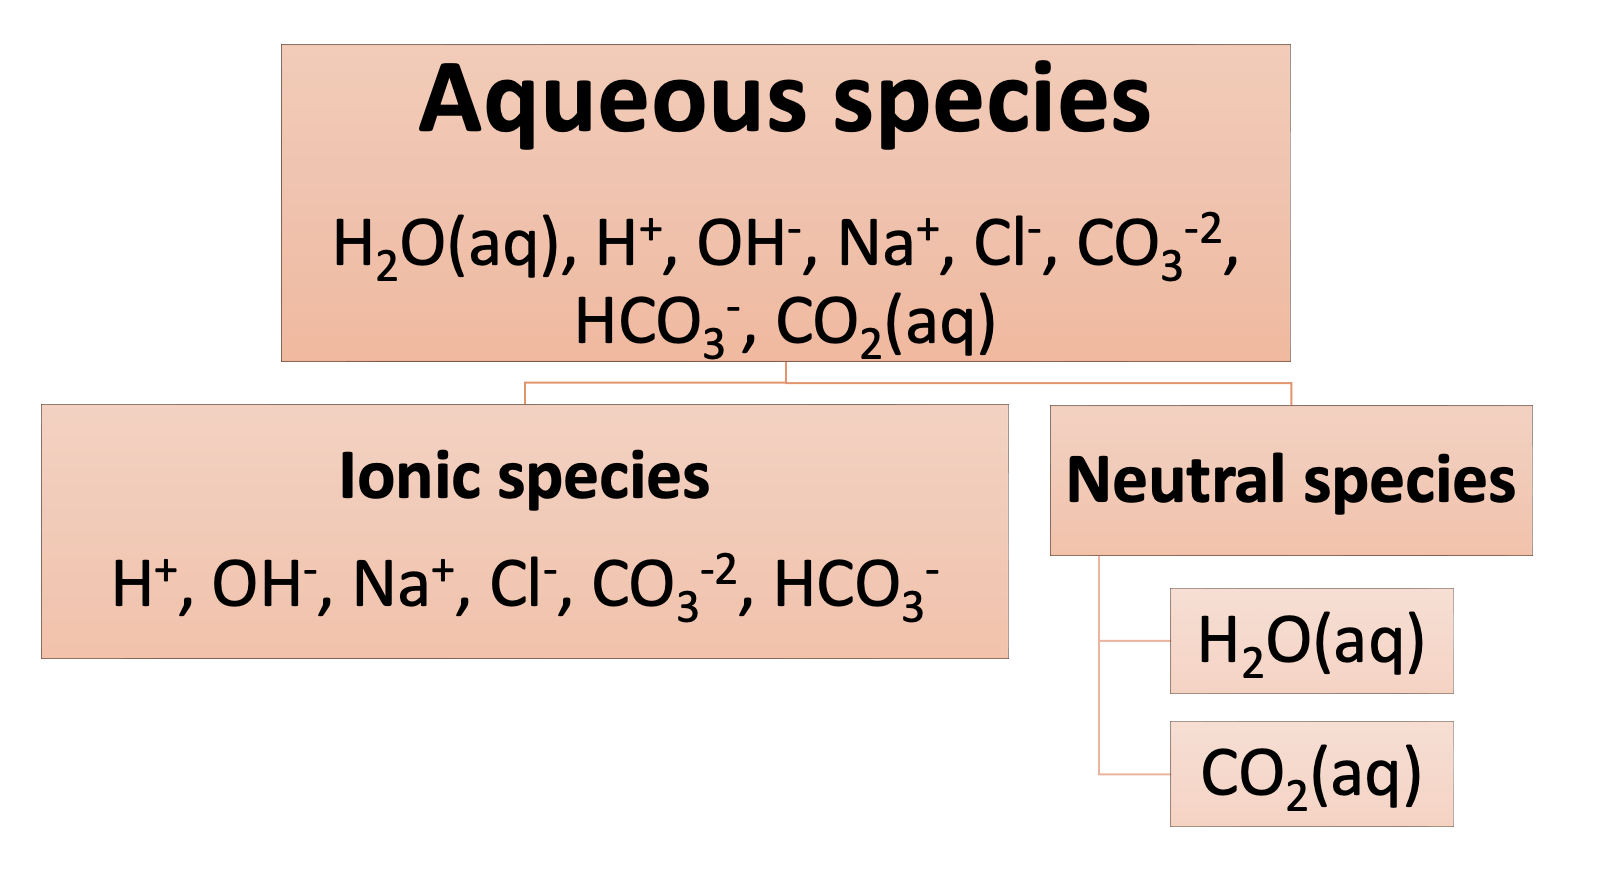
\includegraphics[height=0.9\textheight]{figures/activity-models/activity-aqueous-species-1}
\end{figure}


\end{frame}

\begin{frame}{Activity coefficient of aqueous ionic species, Davies model}
\begin{itemize}[<+->]
\item The \alert{\textbf{Davies activity coefficient model} } calculates $\gamma_{i}$
using:
\[
\boxed{\log_{10}\gamma_{i}=-A_{\gamma}Z_{i}^{2}\left(\dfrac{\sqrt{I}}{1+\sqrt{I}}-0.3I\right),}
\]
where $A_{\gamma}$ is the \textbf{Debye–Hückel parameter} defined as
\[
A_{\gamma}=1.824928\cdot10^{6}\rho_{\mathsf{H_{2}O}}^{1/2}(\epsilon_{\mathsf{H_{2}O}}T)^{-3/2},
\]
%
where $\rho_{\mathsf{H_{2}O}}$ and $\epsilon_{\mathsf{H_{2}O}}$
are the \textbf{density} and \textbf{dielectric constant of pure water} resp. 
\item For 25~°C and 1~bar, $A_{\gamma}=0.5095$.
\item \textbf{Limitations of the model}: 
It is accurate for $I$ is in the range 0.1–0.7 molal, which is equivalent to 1 kg of water mixed with 5.8–40.9 grams of NaCl (0.5-4 teaspoons of table salt).
\end{itemize}
\end{frame}
%
% --------------------------------------------------------------------------------------------------------------------%
% Activity coefficient model for aqueous ionic species: Davies model 
% --------------------------------------------------------------------------------------------------------------------%
%
\begin{frame}{Activity coefficient of aqueous ionic species, Davies model, Exercise}

%\vskip 10pt
\begin{itemize}
\item \alert{\textbf{Quiz:}} What is the activity coefficient of species Na$^{+}$ in an aqueous solution with ionic strength $I=\unit[0.1]{molal}$ using the \emph{Davies activity coefficient model}:
\[
\log_{10}\gamma_{\mathrm{Na^{+}}}=-A_{\gamma}Z_{\mathrm{Na^{+}}}^{2}\left(\dfrac{\sqrt{I}}{1+\sqrt{I}}-0.3I\right), \quad \mbox{where} \quad A_{\gamma}=0.5095?
\]
%
\begin{center}
\href{http://etc.ch/qjLF}{\textcolor{indigo(dye)}{\tt http://etc.ch/qjLF}} \quad or \quad 

\includegraphics[height=0.18\columnwidth]{figures/activity-models/poll-ionic-strength.png}
\end{center}
%
\vskip 10pt
\hiddenpause
\item \textbf{Answer}: 0.7814.
\pause
\item \textbf{Question}: Based on the calculated-above $\gamma_{\mathrm{Na^{+}}}$, is an \emph{ideal solution assumption} with $\gamma_{i}=1$ a reasonable one?
\end{itemize}
\end{frame}
%
% --------------------------------------------------------------------------------------------------------------------%
% Activity coefficient model for aqueous ionic species: Davies model
% --------------------------------------------------------------------------------------------------------------------%
%
\begin{frame}{Activity coefficient as a function of $I$, Davies model}

\begin{figure}
\centering{}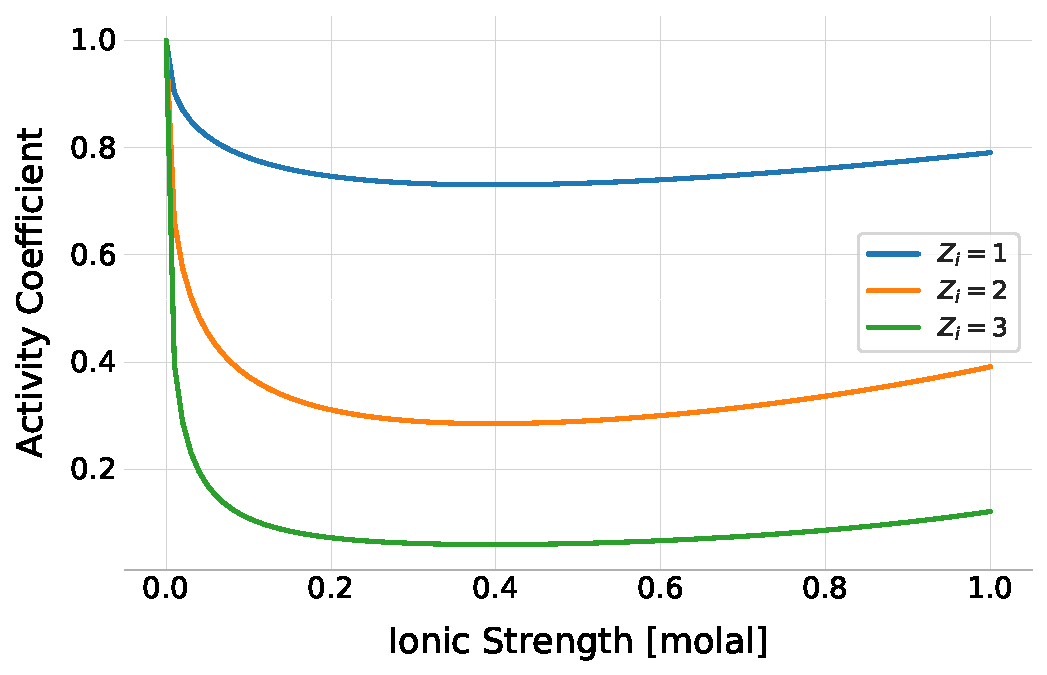
\includegraphics[height=0.7\textheight]{figures/activity-models/activity-coefficient-davies}
\caption*{Activity coefficient $\gamma_{i}$ for aqueous ions with charge $Z_{i}=1,2,3$ as a function of $I$.}
\end{figure}
%
\textbf{Question:} How would these curves look like if the charges would be $Z_i$= -1, -2, -3?

\end{frame}
%
% --------------------------------------------------------------------------------------------------------------------%
% Activity coefficient calculation in Python: Davies model
% --------------------------------------------------------------------------------------------------------------------%
%
\begin{frame}[fragile, allowframebreaks]{Activity coefficient calculation in Python, Davies model}

\lstinputlisting[language=Python, caption=Davies activity model calculation in Python]{python-files/davies-activity-model.py}

Source code: \href{https://polybox.ethz.ch/index.php/s/D0gfkcE1KBiFVxD}{\textcolor{indigo(dye)}{\it davies-activity-model.py}}

\end{frame}
%
\subsubsection{Activity coefficient model for H$_2$O(aq), Davies model}
%
% --------------------------------------------------------------------------------------------------------------------%
% Activity coefficient model for H2O: Davies model
% --------------------------------------------------------------------------------------------------------------------%
%
\begin{frame}{Activity model for H$_{\boldsymbol{2}}$O(aq), Davies model}
\begin{itemize}
\item The \textbf{activity of H$_{2}$O(aq)} can be calculated
using the following \alert{\textbf{Davies model}}:
\[
\boxed{\ln a_{\mathsf{H_{2}O\text{(aq)}}}=\tfrac{\ln10}{55.5084}A_{\gamma}\left[2\left(\tfrac{I+2\sqrt{I}}{1+\sqrt{I}}\right)-4\ln(1+\sqrt{I})-0.3I^{2}\right]-\tfrac{1-x_{\mathsf{\mathsf{H_{2}O\text{(aq)}}}}}{x_{\mathsf{\mathsf{H_{2}O\text{(aq)}}}}}},
\]
where $x_{\mathsf{H_{2}O\text{(aq)}}}$ is the mole fraction of H$_{2}$O(aq):{\small{}
\[
x_{\mathsf{H_{2}O\text{(aq)}}}=\tfrac{n_{\mathsf{H_{2}O\text{(aq)}}}}{\text{sum of moles of all aqueous species}}.
\]
}{\small\par}
\pause
\item \alert{\textbf{Question}}: Consider pure water as a solution.
What is the value of ionic strength $I$ and the activity of water $a_{\sf H_2O}$ ?  
\begin{center}
	\href{http://etc.ch/qjLF}{\textcolor{indigo(dye)}{\tt http://etc.ch/qjLF}} \quad or \quad 
	
\includegraphics[height=0.1\columnwidth]{figures/activity-models/poll-ionic-strength.png}
\end{center}
\hiddenpause
\item \textbf{Answer}: $I$ = 0, $a_{\sf H_2O}$ = 1.
%\item \textbf{Note}: The above activity equation can be derived using \alert{\textbf{Gibbs–Duhem equation}}
%\[
%%\sum n_{i}\text{d}\mu_{i}=0\qquad\text{or}\qquad
%\sum n_{i}\text{d}\ln a{}_{i}=0
%\]
%when the Davies model is used for the activities of ionic species.
\end{itemize}
\end{frame}
%
%
% --------------------------------------------------------------------------------------------------------------------%
% Activity coefficient model for H2O: Ideal model
% --------------------------------------------------------------------------------------------------------------------%
%
\begin{frame}{Activity model for H$_{\boldsymbol{2}}$O(aq),  Ideal model}
\begin{itemize}[<+->]
\item For an \alert{\textbf{ideal solution}}, all contribution arising from ionic strength
can be eliminated:
\begin{alignat*}{2}
\ln a_{\mathsf{H_{2}O\text{(aq)}}} 
& =\cancel{\tfrac{\ln10}{55.5084}A_{\gamma}\left[2\left(\tfrac{I+2\sqrt{I}}{1+\sqrt{I}}\right)-4\ln(1+\sqrt{I})-0.3I^{2}\right]}-\tfrac{1-x_{\mathsf{\mathsf{H_{2}O\text{(aq)}}}}}{x_{\mathsf{\mathsf{H_{2}O\text{(aq)}}}}} \\ 
&=-\tfrac{1-x_{\mathsf{\mathsf{H_{2}O\text{(aq)}}}}}{x_{\mathsf{\mathsf{H_{2}O\text{(aq)}}}}}.
\end{alignat*}
%\item This results in the following simpler activity model for $a_{\mathsf{H_{2}O\text{(aq)}}}$:
%\[
%\ln a_{\mathsf{H_{2}O\text{(aq)}}}=-\tfrac{1-x_{\mathsf{\mathsf{H_{2}O\text{(aq)}}}}}{x_{\mathsf{\mathsf{H_{2}O\text{(aq)}}}}}.
%\]
\item \textbf{Let's investigate how accurate this approximation is?} 
\item \textbf{Source code}: \href{https://polybox.ethz.ch/index.php/s/cAmnV8dKZH7AMcK}{\textcolor{indigo(dye)}{\it activity-water-davies-vs-ideal.py}}.
\end{itemize}
\end{frame}
%
% --------------------------------------------------------------------------------------------------------------------%
% Activity coefficient model for H2O: Davies vs. Ideal model
% --------------------------------------------------------------------------------------------------------------------%
%
\begin{frame}{Activity model for H$_{\boldsymbol{2}}$O(aq): Davies vs. Ideal model}
%
 \lcol
\begin{figure}
\centering
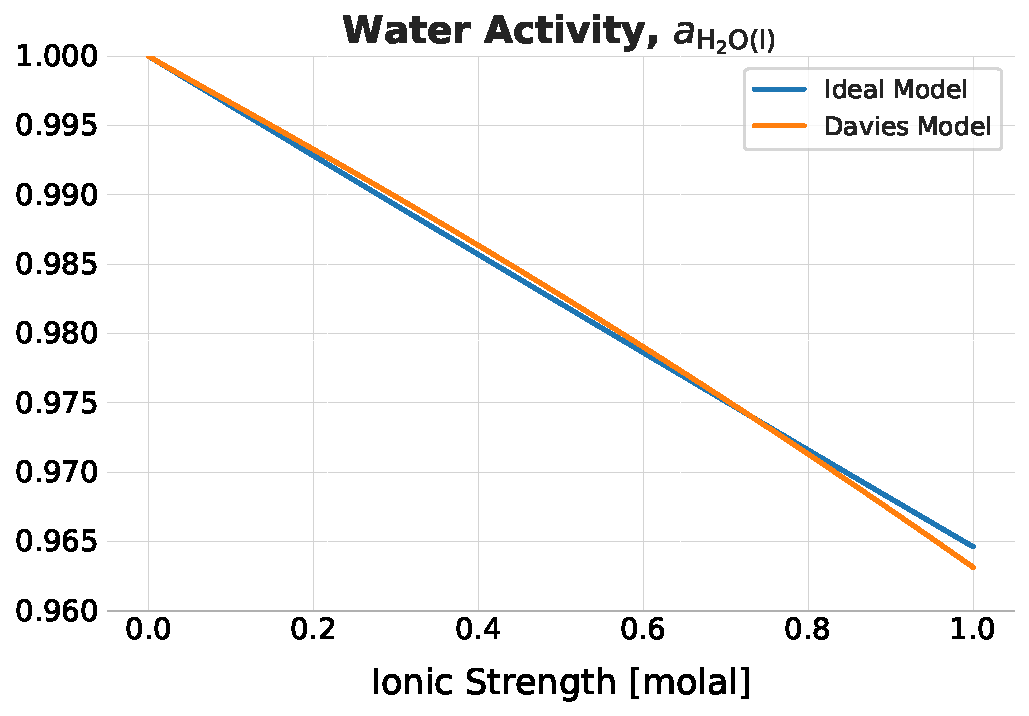
\includegraphics[height=0.73\columnwidth]{figures/activity-models/activity-water-davies-vs-ideal}
\caption{Activities of aqueous solvent species H$_{2}$O(aq) as a function of
ionic strength $I$ calculated using the Ideal and Davies models.}
\end{figure}
\rcol

\begin{figure}
\centering
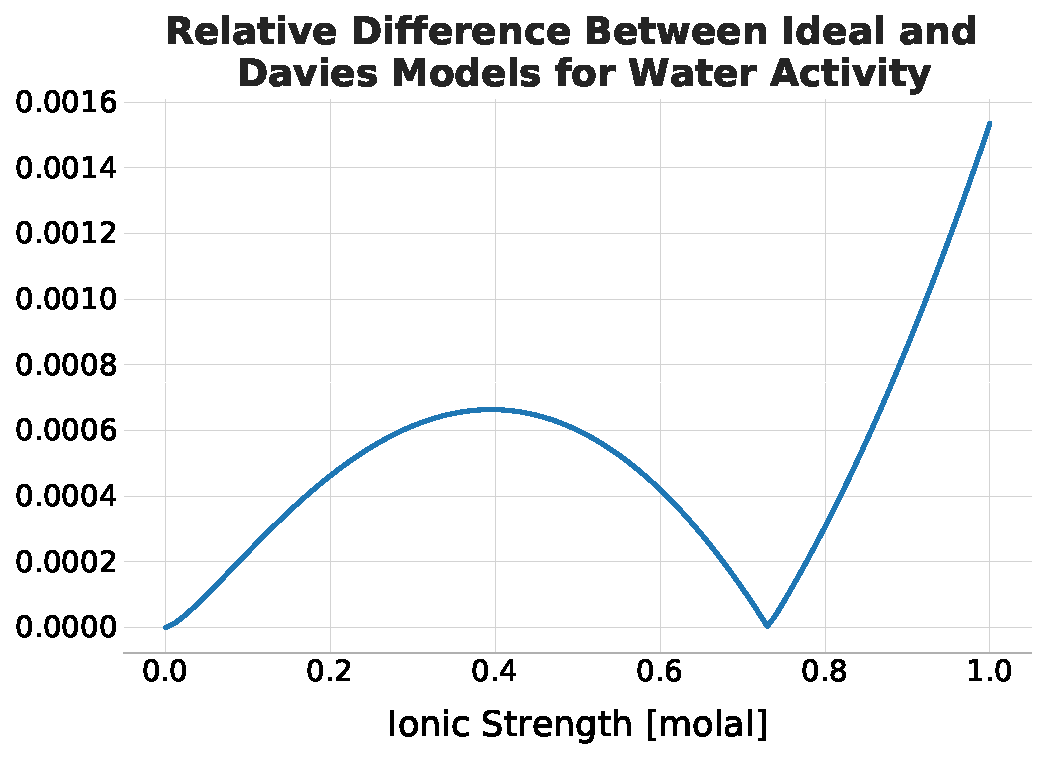
\includegraphics[height=0.73\columnwidth]{figures/activity-models/activity-water-davies-vs-ideal-diff}
\caption{Relative difference between the Ideal and Davies models for activity
of water as a function of ionic strength, $I$.}
\end{figure}
\ecol

\end{frame}
%
\subsubsection{Activity coefficient model for CO$_2$(aq), Drummond model}
%
% --------------------------------------------------------------------------------------------------------------------%
% Activity coefficient model for CO$_{2}$(aq), Drummond model
% --------------------------------------------------------------------------------------------------------------------%
%
\begin{frame}{Activity coefficient model for CO$_{2}$(aq), Drummond model}
\begin{itemize}[<+->]
\item The \textbf{activity of the aqueous species CO$_{2}$(aq)} can be calculated
using
\[
a_{\mathsf{CO_{2}\text{(aq)}}}=\gamma_{\mathsf{CO_{2}\text{(aq)}}}m_{\mathsf{CO_{2}\text{(aq)}}},
\]
with $\gamma_{\mathsf{CO_{2}\text{(aq)}}}$ calculated using the \alert{\textbf{Drummond model}}
\[
\boxed{\ln\gamma_{\mathsf{CO_{2}\text{(aq)}}}=\left(c_{1}+c_{2}T+\tfrac{c_{3}}{T}\right)I-(c_{4}+c_{5}T)\tfrac{I}{I+1}},
\]
where $T$ is temperature,  
$I$ is the ionic strength of the aqueous solution, and 
${c_{1}=-1.0312}$, ${c_{2}=1.2806\cdot10^{-3}}$, ${c_{3}=255.9}$,
${c_{4}=0.4445}$ and ${c_{5}=-1.606\cdot10^{-3}}$. 
\item \textbf{Limitations of the model}: This equation is valid within the temperature and salinity ranges
20–400~°C and 0–6.5~molal, respectively.
\end{itemize}
\end{frame}
%
% --------------------------------------------------------------------------------------------------------------------%
% Calculating the activity coefficient of CO2(aq) in Python
% --------------------------------------------------------------------------------------------------------------------%
%
\begin{frame}[fragile, allowframebreaks]{Calculating CO$_{2}$(aq) activity coefficient using Drummond model in Python}

\lstinputlisting[language=Python, caption=Calculating CO$_{2}$(aq) activity coefficient in Python]{python-files/activity-coefficient-co2-drummond.py}

\textbf{Source code}: \href{https://polybox.ethz.ch/index.php/s/Cg91f6PR1xIuKzY}{\textcolor{indigo(dye)}{\it  activity-coefficient-co2-drummond.py}}.

\end{frame}
%
% --------------------------------------------------------------------------------------------------------------------%
% Drummond activity coefficient model for CO$_{2}$(aq)
% --------------------------------------------------------------------------------------------------------------------%
%
\begin{frame}{Activity coefficient model for CO$_{2}$(aq), Drummond model}

\begin{figure}
\centering{}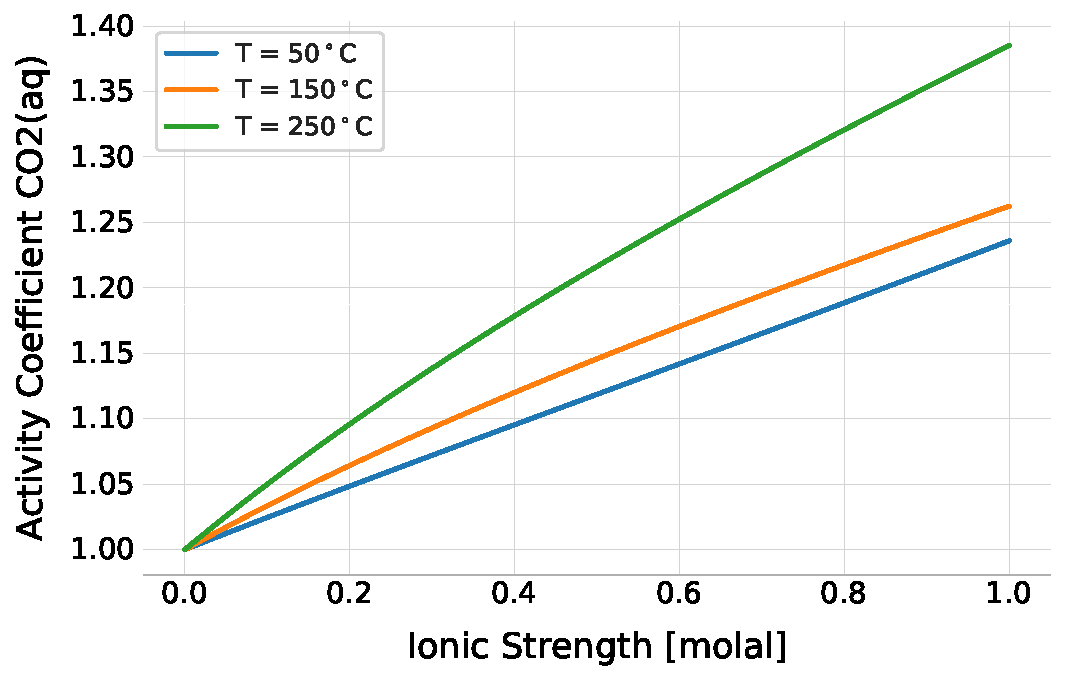
\includegraphics[height=0.8\textheight]{figures/activity-models/activity-coefficient-co2-drummond}
\caption{Activity coefficient of CO$_{2}$(aq) calculated using Drummond model
at temperatures 50, 150, and 250 °C as a function of ionic strength.}
\end{figure}

\end{frame}
%
%
% --------------------------------------------------------------------------------------------------------------------%
% Salting-out effect
% --------------------------------------------------------------------------------------------------------------------%
%
\begin{frame}[<+->]{Salting-out effect}

\small
\begin{itemize}
\item Consider the dissolution reaction for CO$_{2}$(g):
\[
\mathsf{CO_{2}\text{(g)}}\rightleftharpoons\mathsf{CO_{2}\text{(aq)}}.
\]
\item At equilibrium, the following \textbf{mass action equation} is satisfied, i.e., 
%
$K(T, P) := \tfrac{a_{\mathsf{CO_{2}\text{(aq)}}}}{a_{\mathsf{CO_{2}\text{(g)}}}}$.
%\]
\item Combining $a_{\mathsf{CO_{2}\text{(aq)}}} = K(T, P) \, a_{\mathsf{CO_{2}\text{(g)}}}$ and 
$a_{\mathsf{CO_{2}\text{(aq)}}}=\gamma_{\mathsf{CO_{2}\text{(aq)}}}m_{\mathsf{CO_{2}\text{(aq)}}}$, we obtain 
\[
m_{\mathsf{CO_{2}\text{(aq)}}}=\tfrac{1}{\gamma_{\mathsf{CO_{2}\text{(aq)}}}} \, K(T, P) \, a_{\mathsf{CO_{2}\text{(g)}}}(T, P)
\approx \tfrac{1}{\gamma_{\mathsf{CO_{2}\text{(aq)}}}} \, f(T, P).
\]
\item \alert{\textbf{Quiz}}: What happens to $m_{\mathsf{CO_{2}\text{(aq)}}}$ when $\gamma_{\mathsf{CO_{2}\text{(aq)}}}$
increases with $I$ for constant $(T, P)$?
\begin{center}
	\href{http://etc.ch/qjLF}{\textcolor{indigo(dye)}{\tt http://etc.ch/qjLF}} \quad or \quad 
	
\includegraphics[height=0.14\columnwidth]{figures/activity-models/poll-ionic-strength.png}
\end{center}
\hiddenpause
\item \textbf{Answer:} $m_{\mathsf{CO_{2}\text{(aq)}}}$ decrease. 
\end{itemize}
\end{frame}
%
% --------------------------------------------------------------------------------------------------------------------%
% Summary on the calculation of activities of gaseous species
% --------------------------------------------------------------------------------------------------------------------%
%
\begin{frame}[shrink=10]{Summary on the calculation of activities of aqueous species}
	\begin{columns}[t]
		\column{0.5\textwidth}
		\vskip 20pt
		\begin{itemize}[<+->]
			\item  The \alert{activities} of aqueous solute species 
			\[
			a_{i}=\gamma_{i}m_{i}.
			\]
			\item The \alert{molality} of the species 
			\[
			m_{i}=55.508\tfrac{n_{i}}{n_{\mathsf{H_{2}O(aq)}}}.
			\]
			\item The \alert{ionic strength} of the aqueous solution 
			\[
			I=\tfrac{1}{2}\sum_{i}m_{i}Z_{i}^{2}.
			\]
		\end{itemize}
		
		\column{0.5\textwidth}
		\begin{itemize}[<+->]
			\item  The \alert{activity coefficient} $\gamma_{i}$  for  \alert{ionic species} according to the Davies model:
			\[
			\log_{10}\gamma_{i}=-A_{\gamma}Z_{i}^{2}\left(\tfrac{\sqrt{I}}{1+\sqrt{I}}-0.3I\right).
			\]
			\item The \alert{activity of H$_{2}$O(aq)} according to the Davies model:
			\[
			\ln a_{\mathsf{H_{2}O\text{(aq)}}}=-\tfrac{1-x_{\mathsf{\mathsf{H_{2}O\text{(aq)}}}}}{x_{\mathsf{\mathsf{H_{2}O\text{(aq)}}}}}.
			\]
			\item The \alert{activity coefficient} $\gamma_{i}$ for  \alert{CO$_{2}$(aq)} according to the Drummond model:
			\[
			\ln\gamma_{i}=\left(c_{1}+c_{2}T+\tfrac{c_{3}}{T}\right)I-(c_{4}+c_{5}T)\tfrac{I}{I+1}.
			\]
			
		\end{itemize}
	\end{columns}
	
\end{frame}
%
% --------------------------------------------------------------------------------------------------------------------%
% Gaseous phase
% --------------------------------------------------------------------------------------------------------------------%
%
\subsection{Gaseous phase}
%\begin{frame}{}
%\centering
%\Large
%\textbf{Gaseous phase}
%\end{frame}
%
% --------------------------------------------------------------------------------------------------------------------%
% Activities of species in a gaseous solution
% --------------------------------------------------------------------------------------------------------------------%
%
\begin{frame}{Activities of species in a gaseous solution}
\begin{itemize}
\item The \alert{\textbf{activity of gaseous species $i$}} can be calculated using:
\[
\boxed{a_{i}=\varphi_{i}x_{i}\tfrac{P}{P^{\circ}}},
\]
where 
\begin{itemize}
\item $\varphi_{i}$ is the \textbf{fugacity coefficient} of the gaseous species,
\item $x_{i}$ is the \textbf{mole fraction} of the gaseous species,
\item $P$ is pressure (in units of bar, with $\unit[1]{\mathsf{bar}}=\unit[10^{5}]{\mathsf{Pa}}$),
and 
\item $P^{\circ}$ is a reference pressure, $P^{\circ}=\unit[1]{\mathsf{bar}}$.
\end{itemize}
\pause
\item The \textbf{fugacity coefficients of ideal gases} are $\varphi_{i}=1$. \textbf{But}: the gases rarely behaving ideal.  
\end{itemize}
\end{frame}
%
% --------------------------------------------------------------------------------------------------------------------%
% Activity of CO2(g) using a cubic equation of state
% --------------------------------------------------------------------------------------------------------------------%
%
\begin{frame}{Activity of CO$_{\boldsymbol{2}}$(g) using a cubic equation of state}
\begin{itemize}
\item An \textbf{ideal gas} solution has \alert{\textbf{a $PVT$ behavior}} defined by the equation:
\[
\tfrac{PV}{RT}=1,
\]
where $P$ is pressure (in units of Pa), $T$ is temperature (in units
of K), $V$ is molar volume (in units of m$^{3}$/mol), and $R=\unit[8.314]{\mathsf{J/(mol\cdot K)}}$.
\pause
\item For \textbf{real gases}, we introduce a \alert{\textbf{compressibility factor}} $Z$ defined as
%
\[
Z=\tfrac{PV}{RT} < 1.
\]
\pause
\item For \textbf{real gases}, $Z \to 1$ only when
\begin{itemize}
\item temperatures are very high or
\item pressures are very low.
\end{itemize}
\end{itemize}
\end{frame}
%
% --------------------------------------------------------------------------------------------------------------------%
% Compressibility factor of gases
% --------------------------------------------------------------------------------------------------------------------%
%
\begin{frame}{Compressibility factor of gases \, i}

\begin{figure}
\begin{centering}
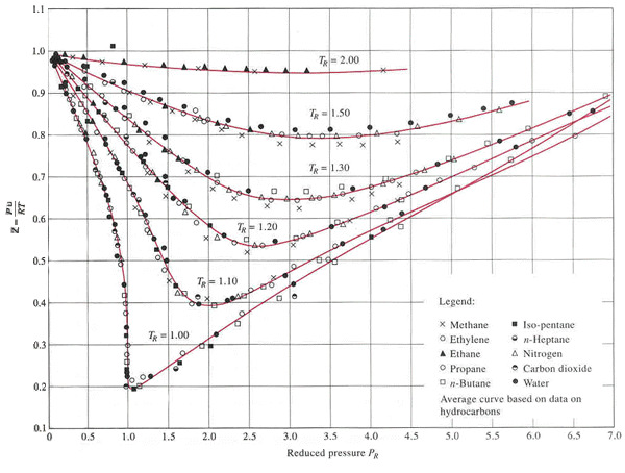
\includegraphics[height=0.8\textheight]{figures/activity-models/compressibility-factor-several-gases}
\par\end{centering}
\caption{{\footnotesize{}The compressibility factor $Z$ as a function of reduced pressure $P_{R} = P/P_{\mathsf{critical}}$
for several reduced temperatures $T_{R} = T/T_{\mathsf{critical}}$ (Cengel and Boles, 2011).}}
\end{figure}

\end{frame}
%
% --------------------------------------------------------------------------------------------------------------------%
% Compressibility factor of gases
% --------------------------------------------------------------------------------------------------------------------%
%
\begin{frame}{Compressibility factor of gases \, ii}

\begin{itemize}
\item Different gases have similar thermodynamic behavior when
$T$ and $P$ are normalized by their critical values $T_{\mathsf{critical}}$ and $P_{\mathsf{critical}}$, respectively.
\item This allows us to use \textbf{single equation of state} to model the $PVT$ behavior of a gas.
\end{itemize}
%
\begin{figure}
\centering
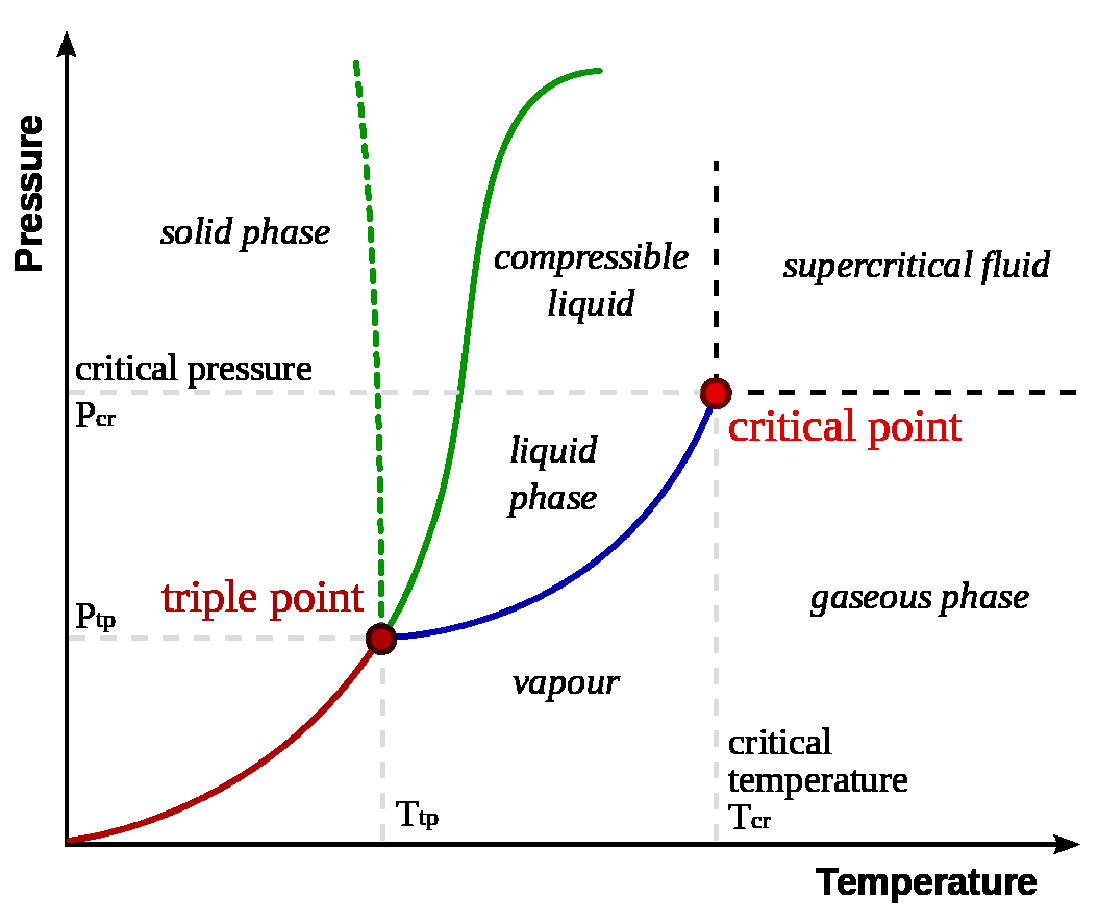
\includegraphics[height=0.6\textheight]{figures/activity-models/phase-diagram-pt}
\caption{{\footnotesize{}A typical phase diagram of a substance. The critical
point is the limit point in the liquid-vapor saturation curve.}}
\end{figure}

%\begin{SCfigure}
%  \centering
%  \caption{A typical phase diagram of a substance. The critical point is the limit point in the liquid-vapor saturation curve.}
%  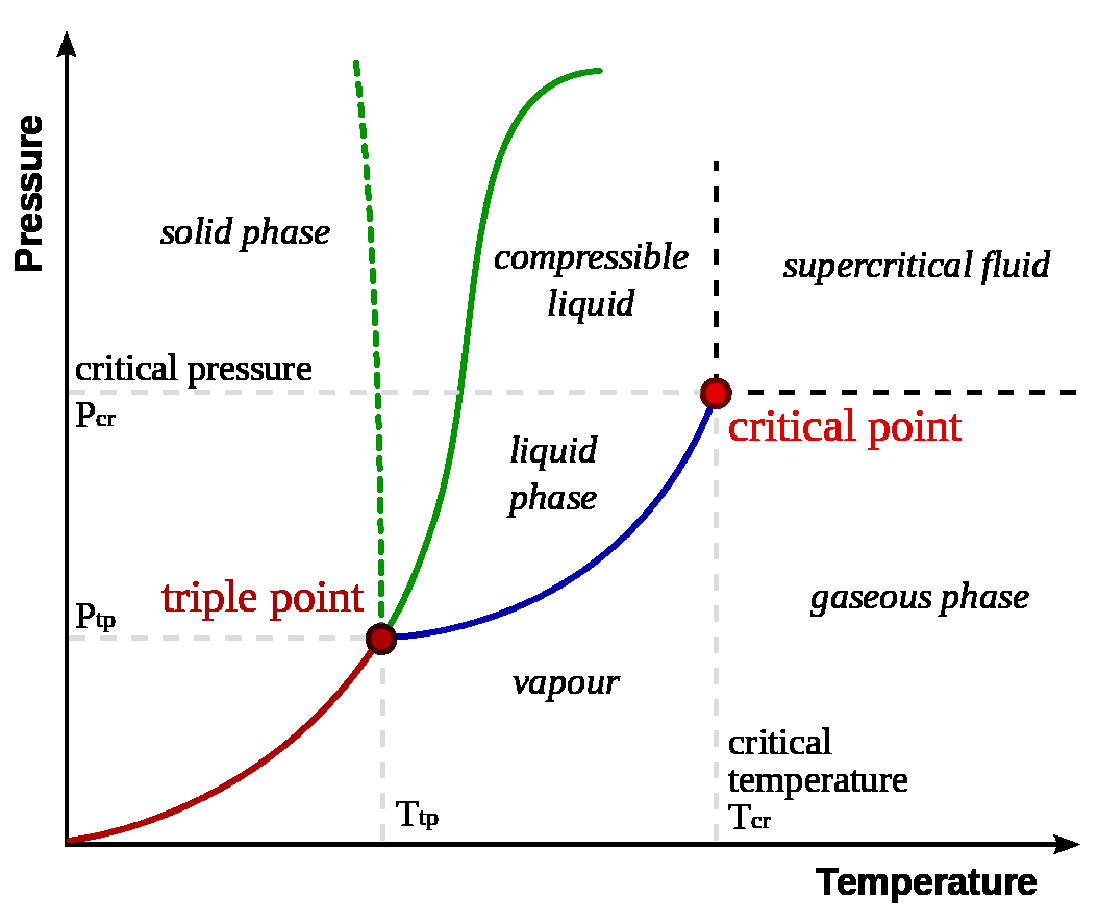
\includegraphics[height=0.6\textheight]{figures/activity-models/phase-diagram-pt}
%  % picture filename
%\end{SCfigure}

%\begin{itemize}
%\end{itemize}

\end{frame}
%
% --------------------------------------------------------------------------------------------------------------------%
% Supercritical carbon dioxide
% --------------------------------------------------------------------------------------------------------------------%
%
\begin{frame}{Supercritical carbon dioxide CO$_{\mathsf{2}}$(g)}
\vskip 5pt
\begin{figure}
\centering
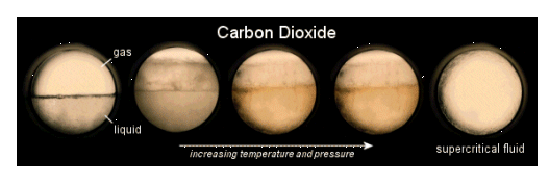
\includegraphics[height=0.45\textheight]{figures/activity-models/subcritical-to-supercritical-co2}
\caption{CO$_{2}$ initially existing in two phases: liquid and gas. As temperature
and pressure increase, it transitions to a state in which there is
only one phase in the \textbf{supercritical state}.}
\end{figure}

\begin{itemize}
\item As a \alert{\textbf{supercritical fluid}}, the substance flows like a gas (less viscous
than liquid) and is dense like a liquid. 
\item In geologic CO$_{2}$ sequestration, the supercritical state is more
advantageous because of its \textbf{high mobility and high density}.
\end{itemize}

\end{frame}
%
% --------------------------------------------------------------------------------------------------------------------%
% Activity of CO2(g) using a cubic equation of state
% --------------------------------------------------------------------------------------------------------------------%
%
\begin{frame}{Cubic equation of state}

\begin{itemize}
\item A \alert{\textbf{general cubic equation of state}} can be written in terms
of $Z$ \citep{Smith2005} as
\[
\boxed{1=\tfrac{1}{Z-\beta}-q\beta\tfrac{1}{(Z+\epsilon\beta)(Z+\sigma\beta)}},
\]
where  
\begin{itemize}
\item $\epsilon$ and $\sigma$ are pure numbers (same for all substances),  
\item $\beta$ and $q$ are  parameters specific to substances and defined as
\[
\beta=\Omega\tfrac{P_{\mathsf{r}}}{T_{\mathsf{r}}} \qquad \mbox{and} \qquad
q=\tfrac{\Psi}{\Omega}\tfrac{\alpha(T_{\mathsf{r}},\omega)}{T_{\mathsf{r}}}
\]
%
with specific to \textbf{a particular equation of state} $\Omega$, $\Psi$, and $\alpha(T)$, 
\item the \textbf{reduced temperature and pressure} $T_{\mathsf{r}} = \tfrac{T}{T_{\mathsf{c}}}$ and
$P_{\mathsf{r}} = \tfrac{P}{P_{\mathsf{c}}}$ are defined via \textbf{critical temperature and pressure} 
$T_{\mathsf{c}}$ and $P_{\mathsf{c}}$, and 
\item $\omega$ is a \alert{acentric factor} that depends on the substance.
\end{itemize}
%
%\item \textbf{Exercise:} Show that the above equation is cubic in $Z$
%by finding the coefficients $A$, $B$, $C$ and $D$ in terms of
%$\beta$, $q$, $\epsilon$ and $\sigma$ of the cubic polynomial:
%\[
%AZ^{3}+BZ^{2}+CZ+D=0.
%\]
%\item \textbf{Note:} more commonly can be found in the form
%%
%\[
%\boxed{P=\tfrac{RT}{V-\beta}-q(T)\beta\tfrac{1}{(V+\epsilon\beta)(V+\sigma\beta)}}.
%\]
\item \textbf{Note:} For CO$_{2}$(g), ${T_{\mathsf{c}}=304.2\;\mathsf{K}}$, ${P_{\mathsf{c}}=73.83\;\mathsf{bar}}$,
${\omega=0.224}$. 
\end{itemize}

\end{frame}
%
%% --------------------------------------------------------------------------------------------------------------------%
%% Activity of CO2(g) using a cubic equation of state 
%% --------------------------------------------------------------------------------------------------------------------%
%%
%\begin{frame}{Activity of CO$_{\boldsymbol{2}}$(g) using a cubic equation of state \, ii}
%\begin{columns}[c]
%
%\column{0.5\textwidth}
%\begin{itemize}
%\item In addition, the \alert{reduced temperature} $T_{\mathsf{r}}$ and
%\alert{reduced pressure} $P_{\mathsf{r}}$ are defined as:
%\[
%T_{\mathsf{r}}=\tfrac{T}{T_{\mathsf{c}}}\qquad\text{and}\qquad P_{\mathsf{r}}=\tfrac{P}{P_{\mathsf{c}}},
%\]
%where $T_{\mathsf{c}}$ and $P_{\mathsf{c}}$ are, respectively, the
%\textbf{critical temperature and pressure} of the substance.
%\item The \alert{acentric factor} $\omega$ is a number that depends on
%the substance.
%\item For CO$_{2}$, ${T_{\mathsf{c}}=304.2\;\mathsf{K}}$, ${P_{\mathsf{c}}=73.83\;\mathsf{bar}}$,
%${\omega=0.224}$. 
%\end{itemize}
%
%\column{0.5\textwidth}
%\begin{overprint}
%\onslide<2>  
%\begin{figure}
%\begin{centering}
%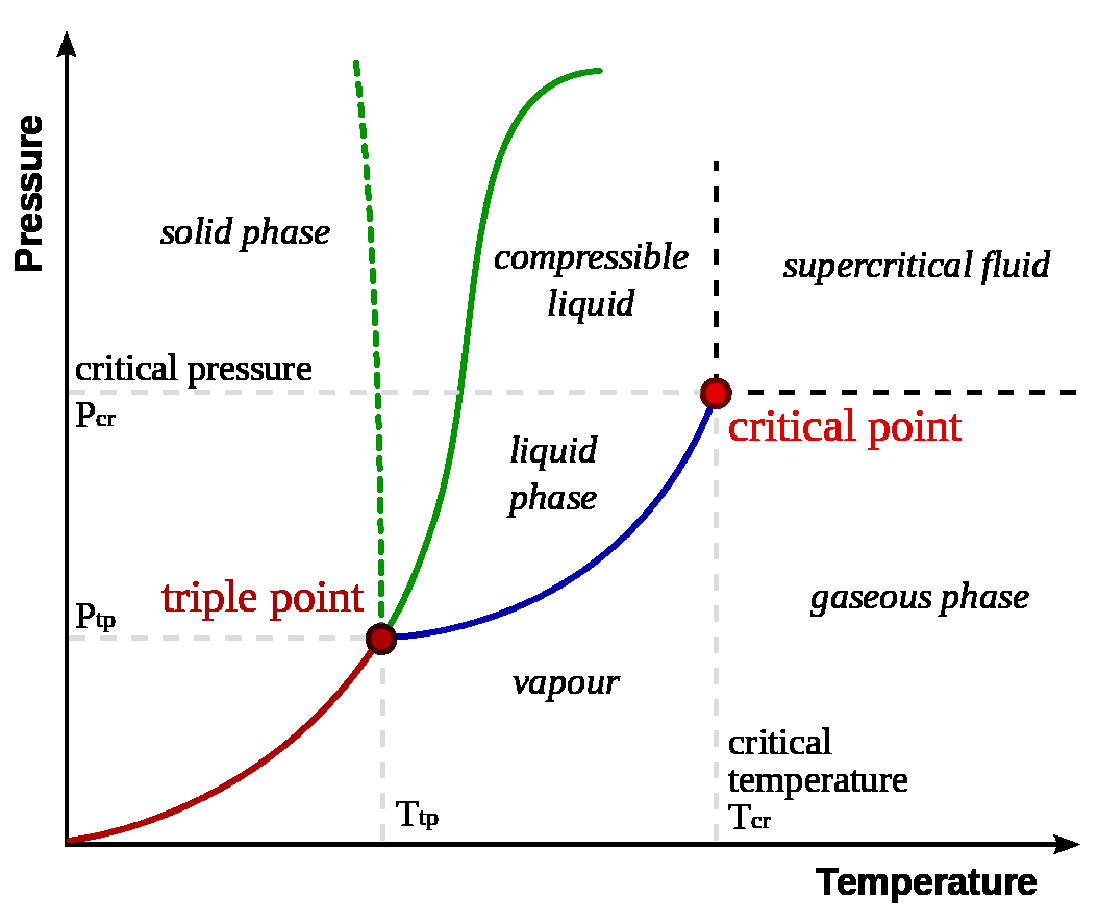
\includegraphics[width=1\textwidth]{figures/activity-models/phase-diagram-pt}
%\par\end{centering}
%\caption{The phase diagram of a substance.}
%\end{figure}
%\end{overprint}
%\end{columns}
%
%\end{frame}
%
% --------------------------------------------------------------------------------------------------------------------%
% Activity of CO2(g) using a cubic equation of state 
% --------------------------------------------------------------------------------------------------------------------%
%
\begin{frame}{Cubic equation of state, Different models \, i}

\begin{table}
\begin{tabular*}{1\textwidth}{@{\extracolsep{\fill}}lcccc}
\toprule 
Equation of State & $\epsilon$ & $\sigma$ & $\Omega$ & $\Psi$\tabularnewline
\midrule 
Ideal Gas & 0 & 0 & 0 & 0\tabularnewline
van der Waals (vdW) $^{1}$ \citeyearpar{VanderWaals1873} & 0 & 0 & 1/8 & 27/64\tabularnewline
Redlich/Kwong (RK) $^{2}$ \citeyearpar{Redlich1949} & 0 & 1 & 0.08664 & 0.42748\tabularnewline
Soave/Redlich/Kwong (SRK) $^{3}$ \citeyearpar{Soave1972} & 0 & 1 & 0.08664 & 0.42748\tabularnewline
\textbf{Peng/Robinson (PR)} $^{4}$ \citeyearpar{Peng1976} & $\mathbf{1-\sqrt{2}}$ & $\mathbf{1+\sqrt{2}}$ & \textbf{0.07780} & \textbf{0.45724} \tabularnewline
\bottomrule
\end{tabular*}

\footnotesize

$^{1}$\citet{VanderWaals1873}; 
$^{2}$\citet{Redlich1949};
$^{3}$\citet{Soave1972}, commonly known as Soave--Redlich--Kwong;
$^{4}$\citet{Peng1976}.

\caption{\normalsize The parameters $\epsilon$, $\sigma$, $\Omega$, and $\Psi$ for different
equation of states.}
\end{table}

\end{frame}
\begin{frame}{Activity of CO$_{\boldsymbol{2}}$(g) using a cubic equation of state \, iii}
	
	\begin{table}
		\begin{tabular*}{1\textwidth}{@{\extracolsep{\fill}}cc}
			\toprule 
			Equation of State & $\alpha(T_{\mathsf{r}},\omega)$\tabularnewline
			\midrule 
			Ideal Gas & 0$\vphantom{\left[T_{\mathsf{r}}^{1/2}\right]^{2}}$\tabularnewline
			van der Waals (vdW) $^{1}$ \citeyearpar{VanderWaals1873} & 1$\vphantom{\left[T_{\mathsf{r}}^{1/2}\right]^{2}}$\tabularnewline
			Redlich/Kwong (RK)$^{2}$ \citeyearpar{Redlich1949} & $T_{\mathsf{r}}^{-1/2}$$\vphantom{\left[T_{\mathsf{r}}^{1/2}\right]^{2}}$\tabularnewline
			Soave/Redlich/Kwong (SRK)$^{3}$ \citeyearpar{Soave1972} & $\left[1+(0.480+1.574\omega-0.176\omega^{2})(1-T_{\mathsf{r}}^{1/2})\right]^{2}$\tabularnewline
			\textbf{Peng/Robinson (PR)} $^{4}$ \citeyearpar{Peng1976} & $\mathbf{\left[1+(0.37464+1.54226\omega-0.26992\omega^{2})(1-T_{\mathsf{r}}^{1/2})\right]^{2}}$\tabularnewline
			\bottomrule
		\end{tabular*}
		
		\footnotesize
		
		\textbf{$^{1}$}\citet{VanderWaals1873}; $^{2}$\citet{Redlich1949};
		$^{3}$\citet{Soave1972}, commonly known as Soave–Redlich–Kwong;
		$^{4}$\citet{Peng1976}.
		
		\caption{The function $\alpha(T_{\mathsf{r}},\omega)$ for different equations of state.}
	\end{table}
	
\end{frame}
%
\begin{frame}{PV phase diagram with isotherms}

\lcol
\begin{itemize}
\item The area in \textbf{green} is a region
in which \textbf{\alert{liquid and vapour coexist}}.
\item There are three \textbf{isothermals}: \alert{\textbf{subcritical}},
\alert{\textbf{critical}}, and \alert{\textbf{supercritical}}. 
\item The horizontal  \textbf{blue segment} corresponds to the fluid change from liquid to vapour at a constant $T$ and $P$. 
\end{itemize}
\rcol

\begin{figure}
\centering 
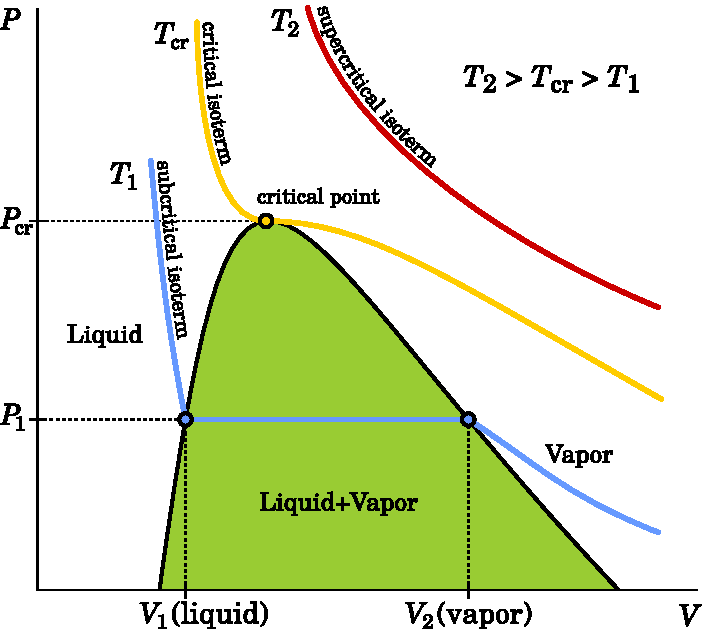
\includegraphics[width=1\textwidth]{figures/activity-models/phase-diagram-pv}
\caption*{\footnotesize Illustration of a $PV$ \textbf{phase diagram} of a substance.}
\end{figure}

\ecol
\end{frame}
%
\begin{frame}{PV phase diagram with isotherms, Roots of cubic EOS \, i}

\lcol
\begin{itemize}
\item Because we are modeling the $PVT$ behavior of a substance
using a \alert{\bf cubic equation of state}:
\[
Z^{3}+AZ^{2}+BZ+C=0,
\]
where $Z=\tfrac{PV}{RT}$ is compressibility factor, 
\textbf{“spurious”} behavior can happen as shown on the next figure.
\item This equation of state has \textbf{utmost three roots}. 
\end{itemize}
\rcol

\begin{figure}
\centering 
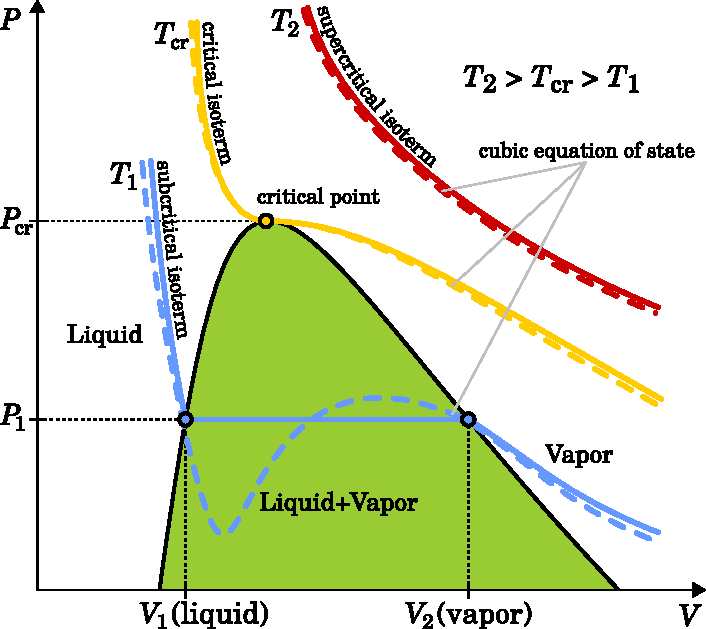
\includegraphics[width=1\textwidth]{figures/activity-models/phase-diagram-pv-cubic-eos}
\caption{\footnotesize Illustration of a $PV$ \textbf{phase diagram} of a substance.}
\end{figure}
\ecol
\end{frame}
%
\begin{frame}{PV phase diagram with isotherms, Roots of cubic EOS \, ii}
\footnotesize
\lcol
\begin{itemize}[<+->]
\item When three real roots exists for cubic equation of state
\begin{itemize}
\item the \textbf{smallest real value} possibly corresponds to the \textbf{liquid state} and 
\item the \textbf{largest real value} possibly corresponds to the \textbf{gaseous state}.
\end{itemize}
\item Any \textbf{root inside the green region} is a \textbf{mathematical artefact} of the cubic model.
%\item Since we are interested in vapour (CO$_{2}$(g)) properties, we will be rather looking at \textbf{the largest 
%root of cubic equation}. 
\item \alert{\textbf{Quiz}}: Which value of $Z$ are we interested
in for CO$_{2}$(g)?
\begin{center}
	\href{http://etc.ch/qjLF}{\textcolor{indigo(dye)}{\tt http://etc.ch/qjLF}} \quad or \quad 
	
\includegraphics[height=0.18\columnwidth]{figures/activity-models/poll-ionic-strength.png}
\end{center} 
\only<6->{
\textbf{Answer}: as we are interested in vapor (CO$_{2}$(g)) properties, we need \textbf{the largest root of cubic EOS}. }
%$T_{\mathrm{cr}}\approx\unit[31.04]{^{\circ}C}$
\end{itemize}
\rcol
\begin{figure}
\centering 
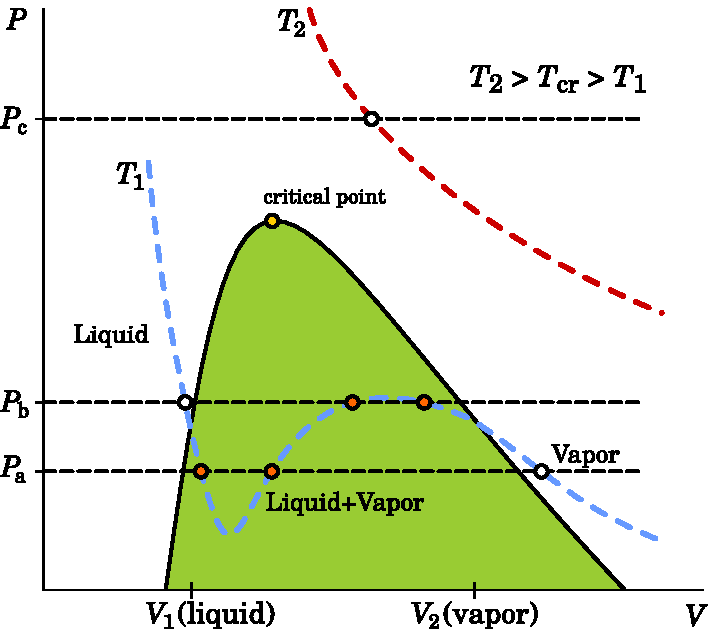
\includegraphics[width=1\textwidth]{figures/activity-models/phase-diagram-pv-cubic-eos-roots}
\caption{\footnotesize Illustration of a $PV$ \textbf{phase diagram} of a substance with roots of cubic equation of state.}
\end{figure}
\ecol
\end{frame}
%
\begin{frame}{Calculating the compressibility factor of CO$_{\boldsymbol{2}}$, Fixed point iteration}
\begin{itemize}
\item The equation of state is non-linear in $Z$, so that its solution requires an \textbf{iterative procedure}.
%
\pause
\item We rearrange it to a more convenient form for \textbf{the largest root} computation \citep{Smith2005}
\[
\boxed{Z = f(Z) = 1+\beta-q\beta\tfrac{Z-\beta}{(Z+\epsilon\beta)(Z+\sigma\beta)}}
\]
and apply simplest iterative approach, the so-called \alert{\textbf{fixed-point iteration method}}: 
\begin{itemize}
\item the \textbf{initial guess} 
\[
Z^{0}=1,
\]
\item the $\boldsymbol{i^{\text{th}}}$ \textbf{iteration}
\[
Z^{i+1} =f(Z^{i})= 1+\beta-q\beta\tfrac{Z^{i}-\beta}{(Z^{i}+\epsilon\beta)(Z^{i}+\sigma\beta)}, 
\]
%
\item the \textbf{acceptance criterion} $|Z^{i+1}-Z^{i}|<\varepsilon$, where $\varepsilon$ is selected tolerance.
\end{itemize}
\end{itemize}
\end{frame}
%
% --------------------------------------------------------------------------------------------------------------------%
% Calculating the compressibility factor of CO2 -- Python code
% --------------------------------------------------------------------------------------------------------------------%
%
\begin{frame}[fragile, allowframebreaks]{Calculating the compressibility factor of CO$_{\boldsymbol{2}}$, Python code}

\lstinputlisting[language=Python, caption=Calculating the compressibility factor of CO2 using fixed point method in Python]{python-files/co2-compressibility-factor-fixed-point.py}

\textbf{Source code}: \href{https://polybox.ethz.ch/index.php/s/39Sznpv0Eirt45B}{\textcolor{indigo(dye)}{\it co2-compressibility-factor-fixed-point.py}}.

\end{frame}
%
\begin{frame}{Calculating the compressibility factor of CO$_{\boldsymbol{2}}$, Fixed point iteration \, i}

\begin{figure}
\begin{centering}
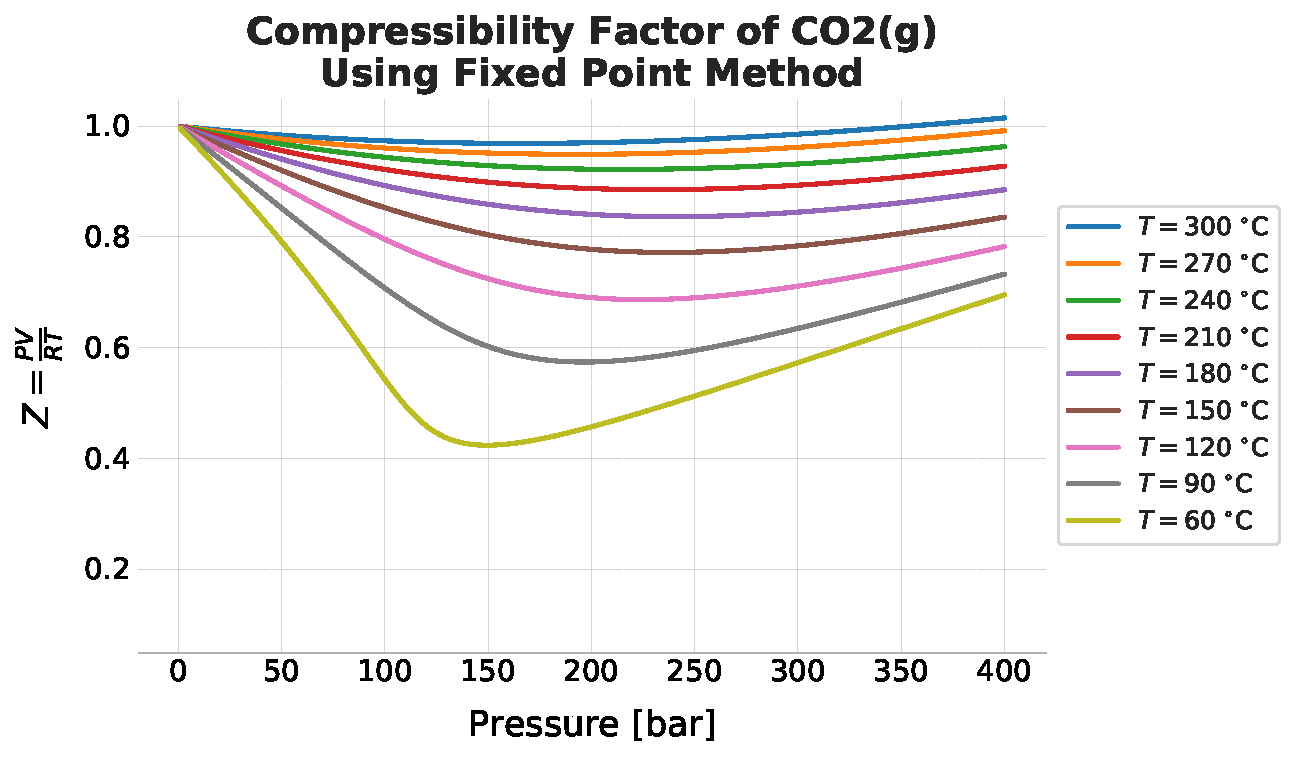
\includegraphics[height=0.8\textheight]{figures/activity-models/co2-compressibility-factor-fixed-point}
\par\end{centering}
\caption*{The compressibility factor $Z$ of CO$_{2}$ for temperatures
60–300 °C and 1–400 bar calculated using \textbf{fixed point iteration method}. }
\end{figure}

\end{frame}
%
% --------------------------------------------------------------------------------------------------------------------%
% Calculating the compressibility factor of CO2 -- Fixed point iteration
% --------------------------------------------------------------------------------------------------------------------%
%
\begin{frame}[fragile]{Calculating the compressibility factor of CO$_{\boldsymbol{\sf 2}}$, Fixed point iteration \, ii}
\begin{columns}[t]

\column{0.5\textwidth}
\begin{itemize}
\item \textbf{Disadvantages} of the fixed point method:\\[-2pt]
\begin{itemize}
\item \textbf{slow}, requiring many iterations; and 
\item \textbf{unstable}, failing to converge. 
\end{itemize}
\pause
\item The fixed point method \textbf{failed at regions close
to the liquid-vapor saturation curve}, for temperatures below
$T_{\sf cr} = $  31.04 °C and pressures close to the saturation pressure (i.e., near the blue curve).
\pause
\item This is due to discontinuity of derivative in the function of Z at $T = T_{\sf cr}$, 
whereas fixed point requires its \alert{\textbf{continuity}}.
\pause
\item \textbf{Solution}: Newton's method.
\end{itemize}

\column{0.5\textwidth}

\begin{figure}
\begin{centering}
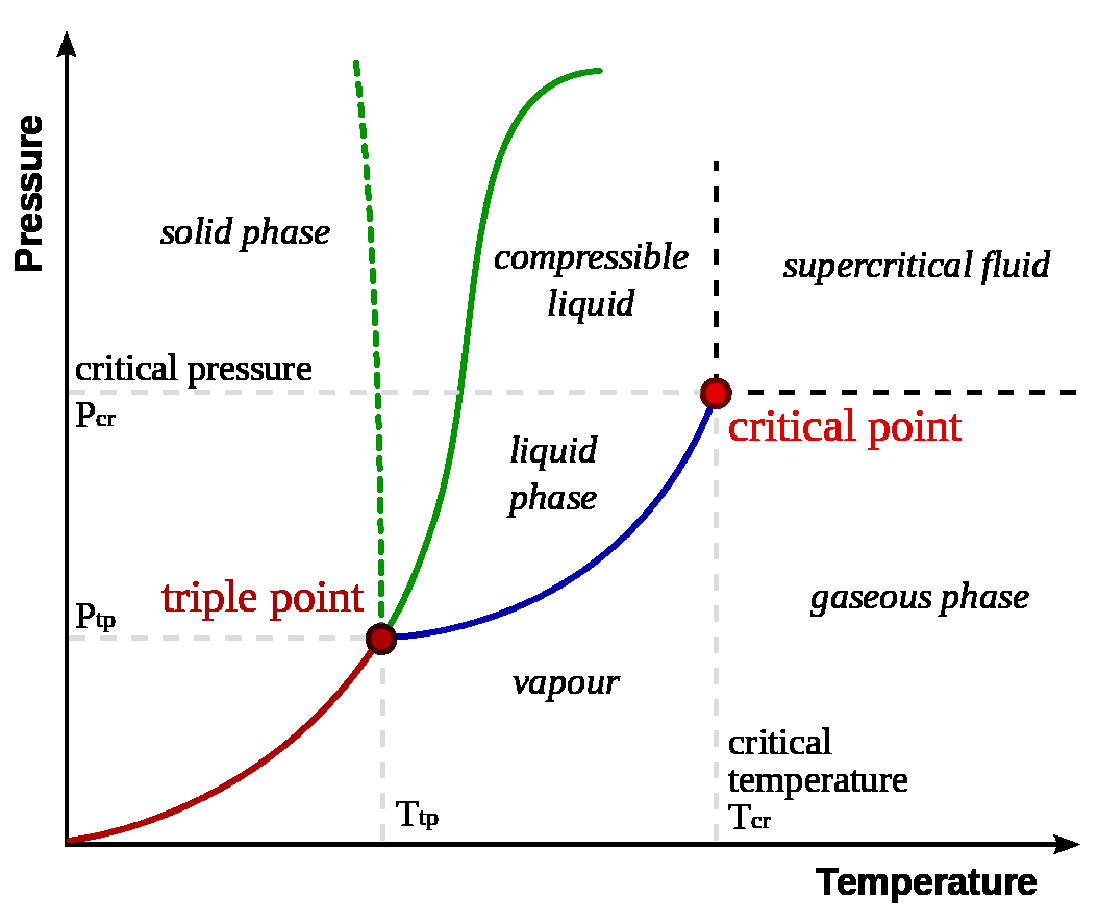
\includegraphics[width=1\columnwidth]{figures/activity-models/phase-diagram-pt}
\par\end{centering}
\caption{The phase diagram of a substance.}
\end{figure}

\end{columns}

\end{frame}
%
% --------------------------------------------------------------------------------------------------------------------%
% Compressibility factor of CO2 -- Newton vs. Fixed point method
% --------------------------------------------------------------------------------------------------------------------%
%
\begin{frame}{Compressibility factor of CO$_{\boldsymbol{2}}$, Newton vs. Fixed point method}
\begin{columns}[t]

\column{0.5\textwidth}

\begin{figure}
\centering
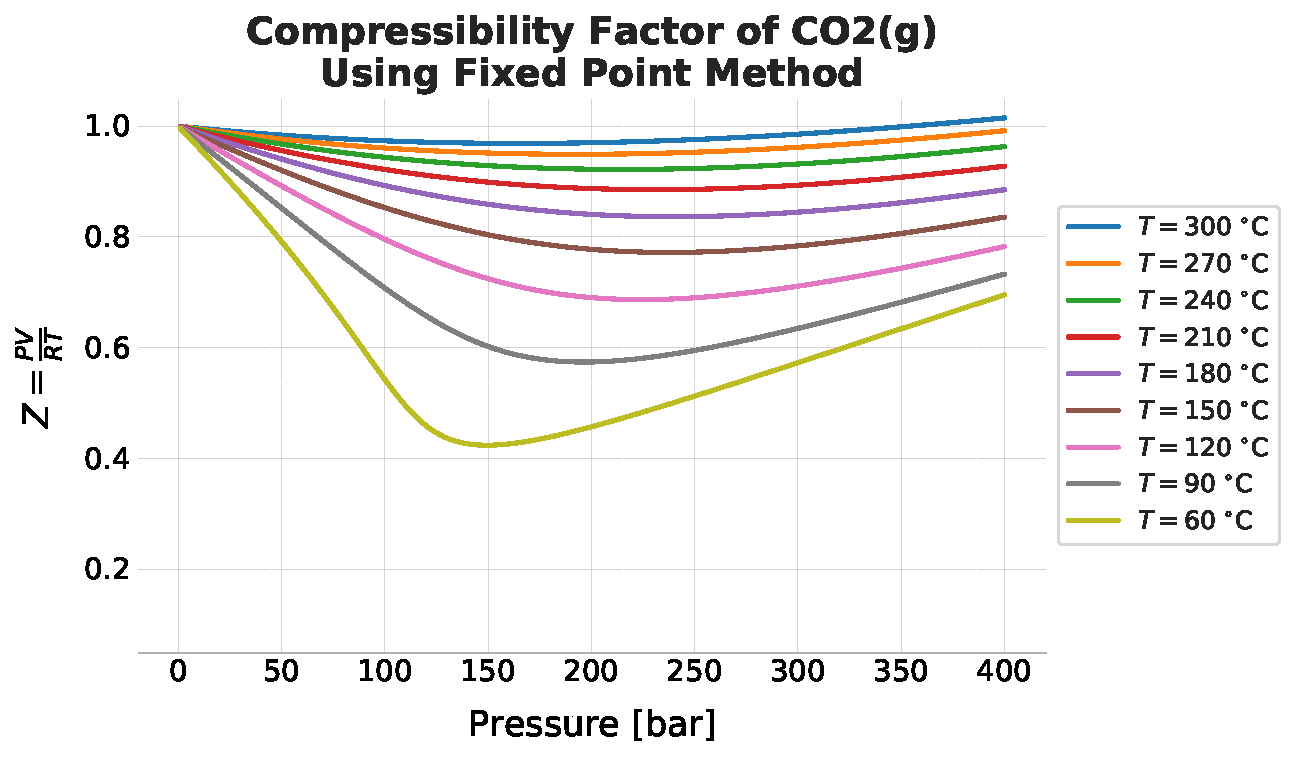
\includegraphics[width=1.05\columnwidth]{figures/activity-models/co2-compressibility-factor-fixed-point}
\caption{The compressibility factor $Z$ of CO$_{2}$ for temperatures
60–300 °C and 1–400 bar using \textbf{fixed point iteration method}.
\alert{\textbf{Failed computations for temperatures 0 and 30 °C!}}}
\end{figure}

\column{0.5\textwidth}

\begin{figure}
\centering
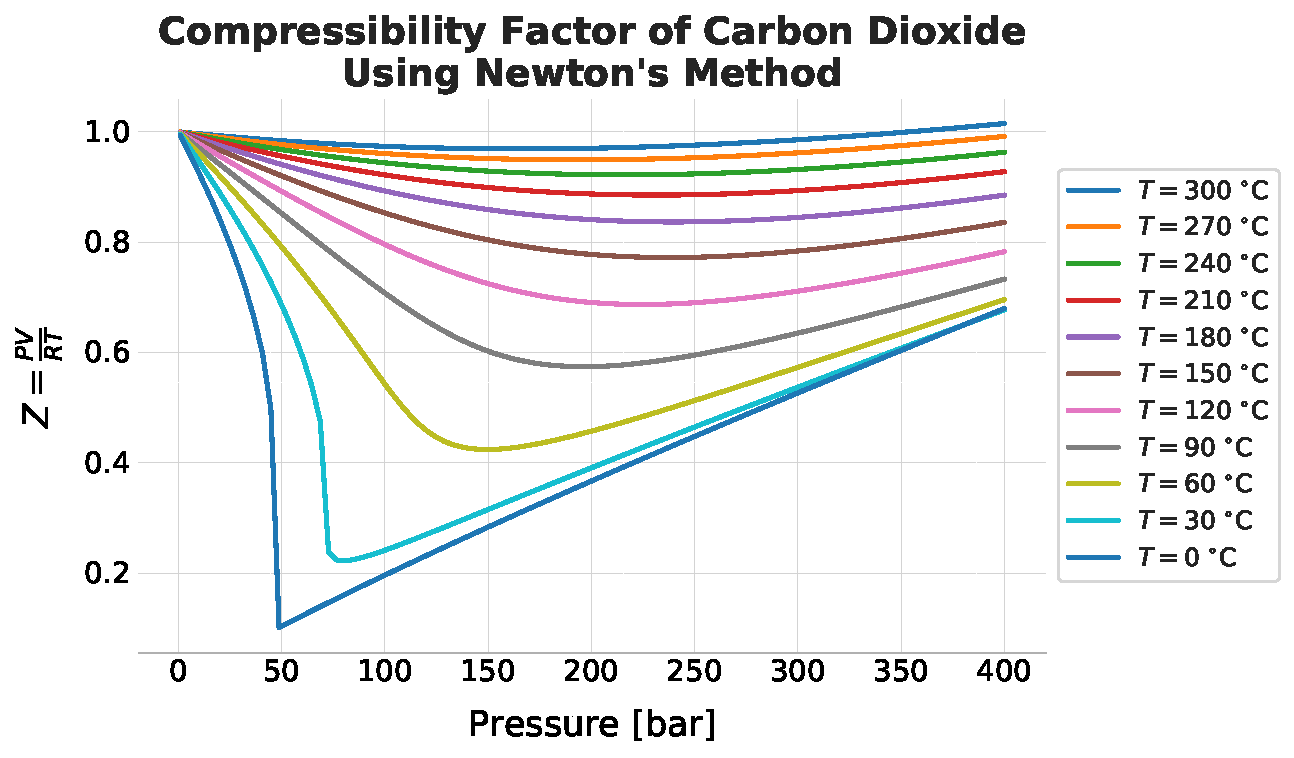
\includegraphics[width=1.05\columnwidth]{figures/activity-models/co2-compressibility-factor-newton}
\caption{The compressibility factor $Z$ of CO$_{2}$ for temperatures
0–300 °C and 1–400 bar using \textbf{Newton's method}. 
\alert{\textbf{Newton's method had no trouble for temperatures 0 and 30 °C!}}}
\end{figure}

\end{columns}
\end{frame}
%
% --------------------------------------------------------------------------------------------------------------------%
% Compressibility factor of CO2 -- Newton's method
% --------------------------------------------------------------------------------------------------------------------%
%
\begin{frame}{Calculating the compressibility factor of CO$_{\boldsymbol{2}}$, Newton's method}
\begin{itemize}
\item In \alert{\textbf{Newton's method}}, we transform the non-linear equation
$Z=1+\beta-q\beta\tfrac{Z-\beta}{(Z+\epsilon\beta)(Z+\sigma\beta)}$
into the form $r(Z)=0$, where $r$ is the \textbf{residual function} 
\[
\boxed{r(Z) 
	= f(Z) - Z 
	= 1+\beta-q\beta\tfrac{Z-\beta}{(Z+\epsilon\beta)(Z+\sigma\beta)}-Z}.
\]
\item Newton's method requires \textbf{first order derivative} of $r(Z)$ in its iterative process:
\begin{itemize}
\item the \textbf{initial guess} 
\[
Z^{0}=1,
\]
\item $\boldsymbol{i^{\text{th}}}$ \textbf{iteration}
\[
Z^{i+1} =Z^{i}-r(Z^{i})/r^{\prime}(Z^{i}),
\]
where 
%
\[
r^{\prime}(Z)=-\tfrac{q\beta}{(Z+\epsilon\beta)(Z+\sigma\beta)}\left\{ 1-(Z-\beta)\tfrac{2Z+(\epsilon+\sigma)\beta}{(Z+\epsilon\beta)(Z+\sigma\beta)}\right\} -1,
\]
%
\item and \textbf{acceptance criterion} $|r(Z^{i+1})|<\varepsilon$, where $\varepsilon$ is selected tolerance.
\end{itemize} 
\end{itemize}
\end{frame}
%
% --------------------------------------------------------------------------------------------------------------------%
% Compressibility factor of CO2 -- Newton's method
% --------------------------------------------------------------------------------------------------------------------%
%
\begin{frame}[fragile, allowframebreaks]{Calculating the compressibility factor of CO$_{\boldsymbol{2}}$, Python code}

\lstinputlisting[language=Python, caption=Calculating the compressibility factor of CO$_{\boldsymbol{2}}$ using Newton's method in Python]{python-files/co2-compressibility-factor-newton.py}

\textbf{Source code}: \href{}{\textcolor{indigo(dye)}{\it polybox}}.

\end{frame}
%
% --------------------------------------------------------------------------------------------------------------------%
% Compressibility factor of CO2 -- Newton's method
% --------------------------------------------------------------------------------------------------------------------%
%
\begin{frame}{Calculating the compressibility factor of CO$_{\boldsymbol{2}}$, Newton's method}
\begin{columns}[t]

\footnotesize
\column{0.61\textwidth}

\begin{figure}
\centering
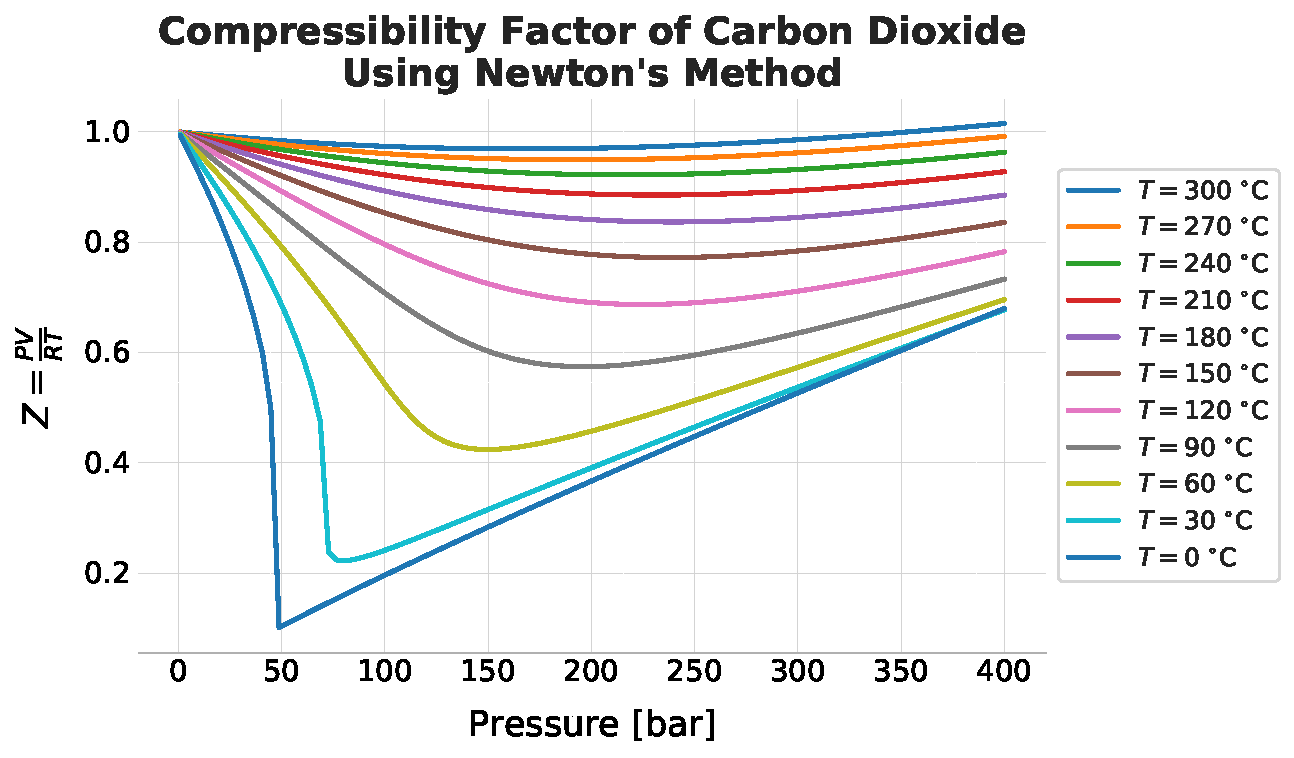
\includegraphics[width=0.8\columnwidth]{figures/activity-models/co2-compressibility-factor-newton}
\caption{For $T < T_{\sf cr} (\mathsf{CO_2})= $ 31.04~°C, the increase in pressure results in a phase transition from vapor to liquid.}
\end{figure}

\column{0.42\textwidth}

\begin{figure}
\centering
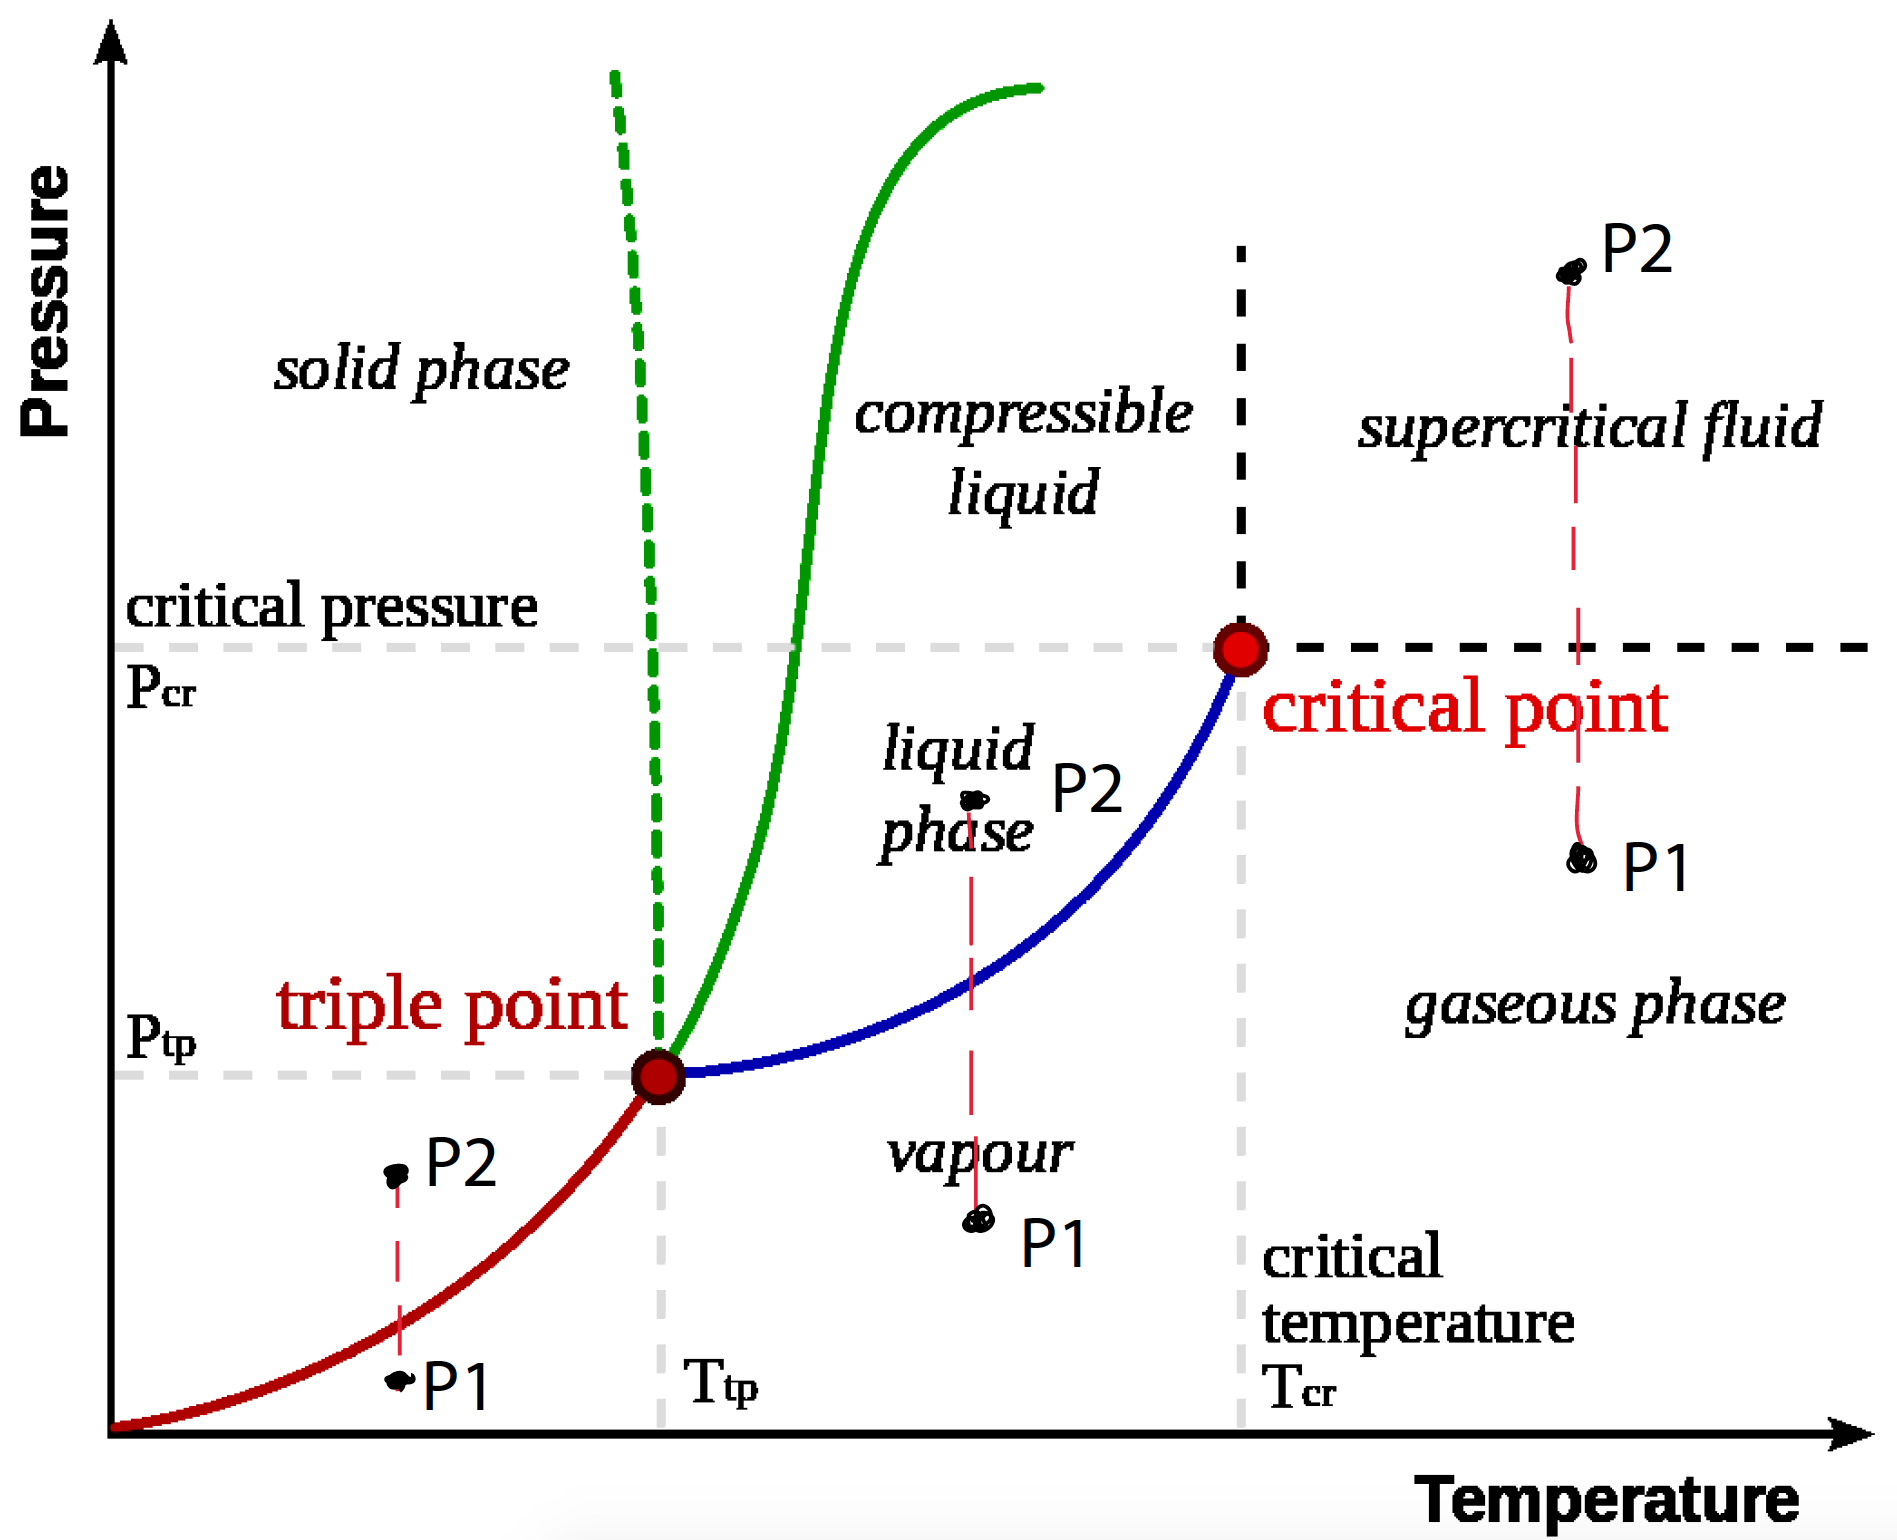
\includegraphics[width=0.8\columnwidth]{figures/activity-models/phase-diagram-pt-with-lines.png}
\caption{The phase diagram of a substance. $T_{\mathrm{cr}}(\mathsf{CO_2})=$  31.04~°C.}
\end{figure}

\end{columns}

\pause
\alert{\textbf{Quiz}}: To which part of the phase diagram does the blue lines correspond to, \\ 
if we are increasing P1 to P2?
\vskip -30pt

\includegraphics[height=0.12\columnwidth, right]{figures/activity-models/poll-ionic-strength.png}
\hiddenpause
\vskip -20pt
\textbf{Answer:} to the middle. 
\end{frame}
%
% --------------------------------------------------------------------------------------------------------------------%
% Activity of CO2 using a cubic equation of state
% --------------------------------------------------------------------------------------------------------------------%
%
\begin{frame}{Activity of CO$_{\boldsymbol{2}}$(g) using a cubic equation of state}
\begin{itemize}
\item Once $Z$ is calculated, the \alert{\textbf{fugacity coefficient of the gas}} is computed
using:
\[
\boxed{\ln\varphi_{i}\coloneqq Z-1-\ln(Z-\beta)-q\theta},
\]
where $\theta$ is defined as:\[
\theta\coloneqq\begin{cases}
{\displaystyle \tfrac{1}{\sigma-\epsilon}\ln\left(\tfrac{Z+\sigma\beta}{Z+\epsilon\beta}\right)} & \epsilon\neq\sigma\\
{\displaystyle \tfrac{\beta}{Z+\epsilon\beta}} & \epsilon=\sigma
\end{cases}
\]
dependent on the equation of state.
\item The \alert{\textbf{activity of CO$_{2}$(g)}} is calculated using:
\[
a_{\mathsf{CO_{2}\text{(g)}}}=\varphi_{\mathsf{CO_{2}\text{(g)}}}\tfrac{P}{P^{\circ}},
\]
with $P$ measured in bar and $P^{\circ}=\unit[1]{\mathsf{bar}}$.
\end{itemize}
\end{frame}
%
% --------------------------------------------------------------------------------------------------------------------%
% Fugacity coefficient of CO2 following the calculation of Z
% --------------------------------------------------------------------------------------------------------------------%
%
\begin{frame}{Fugacity coefficient of CO$_{\boldsymbol{2}}$ following the calculation of $Z$}

\begin{figure}
\begin{centering}
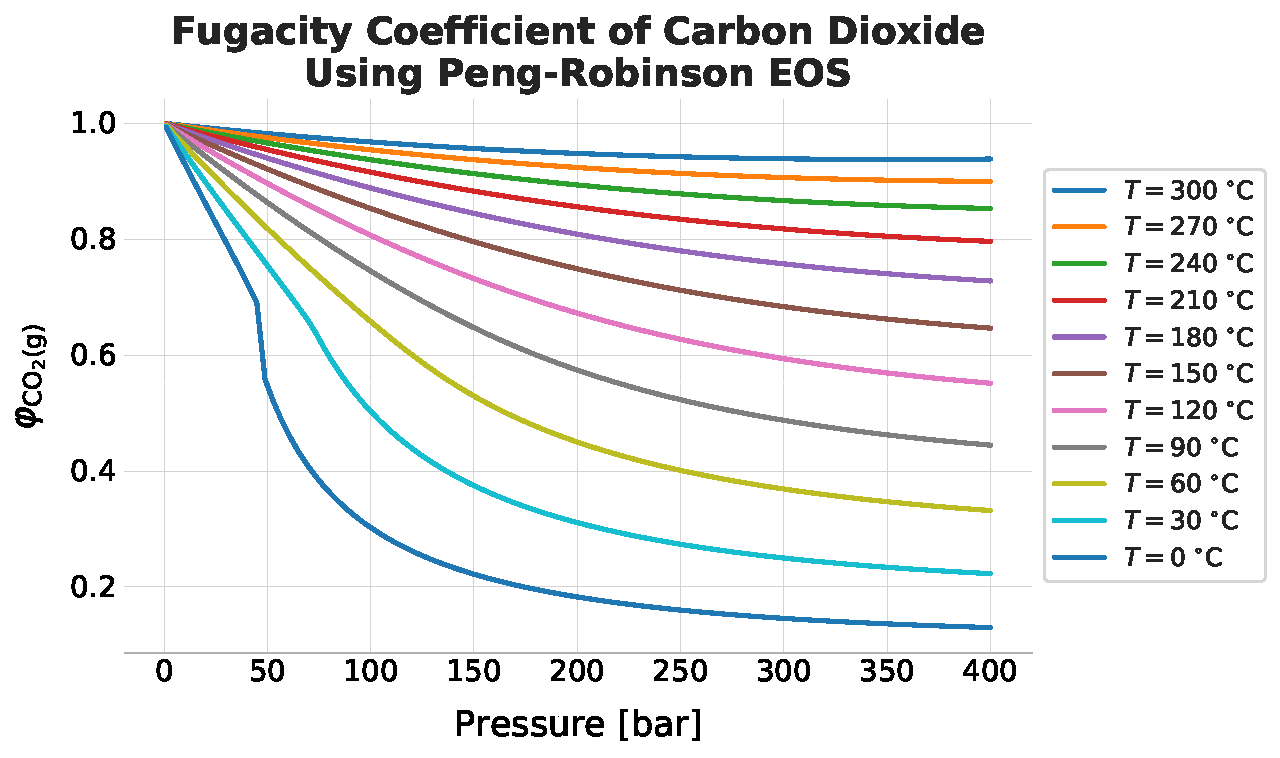
\includegraphics[height=0.8\textheight]{figures/activity-models/fugacity-coefficient-co2-peng-robinson}
\par\end{centering}
\caption{The fugacity coefficient of CO$_{2}$ using Peng--Robinson equation
of state (EOS) for temperatures 0–300 °C and 1–400 bar. }
\end{figure}

\end{frame}
%
% --------------------------------------------------------------------------------------------------------------------%
% Summary on the calculation of activities of gaseous species
% --------------------------------------------------------------------------------------------------------------------%
%
\begin{frame}{Summary on the calculation of activities of gaseous species}
\begin{columns}[t]

\column{0.5\textwidth}
\begin{itemize}[<+->]
\item  The \alert{activities of gaseous species}:
\[
a_{i}=\tfrac{\varphi_{i}x_{i}P}{P^{\circ}}.
\]
%\item We will only consider CO$_{2}$(g) in the gaseous phase, so that the
%\alert{mole fraction} $x_{i}=1$.
\item The \alert{fugacity coefficient} of the CO$_{2}$(g):
\[
\ln\varphi_{i}=Z-1-\ln(Z-\beta)-q\theta
\]
\end{itemize}

\column{0.5\textwidth}
\begin{itemize}[<+->]
\item  The \alert{compressibility factor} 
\[
Z=\tfrac{PV}{RT} < 1
\]
with $Z\equiv1$ \textbf{only} when the substance is an \textbf{ideal gas}.
%
\item Calculation of $Z$ requires the solution of the \alert{cubic equation of state}
\[
Z=\tfrac{Z}{Z-\beta}-q\beta\tfrac{Z}{(Z+\epsilon\beta)(Z+\sigma\beta)}
\]
by \emph{fixed point method} or \emph{Newton's method}.
\end{itemize}
\end{columns}

\end{frame}
%
\subsection{Mineral phase}
%
% --------------------------------------------------------------------------------------------------------------------%
% Summary on the calculation of activities of mineral species
% --------------------------------------------------------------------------------------------------------------------%
%
\begin{frame}{Summary on the calculation of activities of mineral species}
\begin{itemize}
\item The activities of pure minerals (e.g., mineral phases composed by
a single mineral only) is
%
\[
a_{i}=1.
\]
\end{itemize}
\end{frame}
